\documentclass[journal]{IEEEtran}

\usepackage[T1]{fontenc}
\usepackage[utf8]{inputenc}
\usepackage{amsmath,amssymb,amsfonts}
\usepackage{graphicx}
\usepackage{booktabs}
\usepackage{array}
\usepackage{url}
\usepackage{xcolor}
\usepackage{algorithm}
\usepackage{algpseudocode}
\usepackage[hidelinks]{hyperref}
\usepackage{orcidlink}
\usepackage{balance}

\graphicspath{{../figures/}}

\renewcommand{\topfraction}{0.92}
\renewcommand{\bottomfraction}{0.75}
\renewcommand{\textfraction}{0.08}
\renewcommand{\floatpagefraction}{0.80}

% IEEEtran hard-codes an em-dash after the abstract and index-terms names; the CAOS
% content standard (ADR-0067) excludes em-dashes, so the separator is a full stop.
\makeatletter
\def\abstract{\normalfont
    \if@twocolumn
      \@IEEEabskeysecsize\bfseries\textit{\abstractname}.\ \relax
    \else
      \bgroup\par\addvspace{0.5\baselineskip}\centering\vspace{-1.78ex}\@IEEEabskeysecsize\textbf{\abstractname}\par\addvspace{0.5\baselineskip}\egroup\quotation\@IEEEabskeysecsize
    \fi\@IEEEgobbleleadPARNLSP}
\def\IEEEkeywords{\normalfont
    \if@twocolumn
      \@IEEEabskeysecsize\bfseries\textit{\IEEEkeywordsname}.\ \relax
    \else
      \bgroup\par\addvspace{0.5\baselineskip}\centering\@IEEEabskeysecsize\textbf{\IEEEkeywordsname}\par\addvspace{0.5\baselineskip}\egroup\quotation\@IEEEabskeysecsize
    \fi\@IEEEgobbleleadPARNLSP}
\makeatother

% Numbers quoted in the text are read from the committed artifacts by figures/make_figs.py.
% Written by figures/make_figs.py from the committed summaries; do not edit.
\newcommand{\alAhalfS}{0.2\pm1.2}
\newcommand{\alAhalfTen}{-128.9\pm14.5}
\newcommand{\alAhalfW}{1.7\pm1.3}
\newcommand{\alAhalfX}{2.0\pm3.5}
\newcommand{\alAmS}{62.6\pm1.2}
\newcommand{\alAmTen}{-37.4\pm14.0}
\newcommand{\alAmW}{79.6\pm1.4}
\newcommand{\alAmX}{174.1\pm3.6}
\newcommand{\alAoneS}{-20.4\pm1.2}
\newcommand{\alAoneTen}{-154.7\pm18.0}
\newcommand{\alAoneW}{-26.2\pm1.3}
\newcommand{\alAoneX}{-55.8\pm3.3}
\newcommand{\alAtwoS}{-61.4\pm1.2}
\newcommand{\alAtwoTen}{-199.8\pm13.9}
\newcommand{\alAtwoW}{-78.3\pm1.4}
\newcommand{\alAtwoX}{-173.0\pm3.6}
\newcommand{\alAzeroS}{21.0\pm1.2}
\newcommand{\alAzeroTen}{-91.8\pm13.7}
\newcommand{\alAzeroW}{26.2\pm1.4}
\newcommand{\alAzeroX}{60.8\pm3.3}
\newcommand{\alCAhalfS}{0.0}
\newcommand{\alCAhalfW}{0.0}
\newcommand{\alCAhalfX}{0.0}
\newcommand{\alCAmS}{-60.6}
\newcommand{\alCAmW}{-77.5}
\newcommand{\alCAmX}{-60.6}
\newcommand{\alCAoneS}{20.2}
\newcommand{\alCAoneW}{25.8}
\newcommand{\alCAoneX}{20.2}
\newcommand{\alCAtwoS}{60.6}
\newcommand{\alCAtwoW}{77.5}
\newcommand{\alCAtwoX}{60.6}
\newcommand{\alCAzeroS}{-20.2}
\newcommand{\alCAzeroW}{-25.8}
\newcommand{\alCAzeroX}{-20.2}
\newcommand{\alKqS}{-22.1\pm1.2}
\newcommand{\alPlaneTen}{-63.6}
\newcommand{\cFixKwS}{20.2}
\newcommand{\cFixKwW}{25.8}
\newcommand{\cFixTphS}{0.0}
\newcommand{\cFixTphW}{0.0}
\newcommand{\capAffRefitSBig}{1.211}
\newcommand{\capAffSBig}{1.000}
\newcommand{\capAffSTen}{0.966}
\newcommand{\capAffWBig}{1.000}
\newcommand{\capAffWTen}{0.968}
\newcommand{\capAffXBig}{0.998}
\newcommand{\capAffXTen}{0.919}
\newcommand{\capHalfSBig}{0.995}
\newcommand{\capHalfSTen}{0.963}
\newcommand{\capHalfWBig}{1.002}
\newcommand{\capHalfWTen}{0.973}
\newcommand{\capHalfXBig}{1.005}
\newcommand{\capHalfXTen}{0.923}
\newcommand{\capRoMseS}{1.7}
\newcommand{\capRoMseW}{2.0}
\newcommand{\capRoMseX}{4.4}
\newcommand{\capRoRefitSBig}{0.986}
\newcommand{\capRoRefitXTen}{0.621}
\newcommand{\capRoRmseS}{0.8}
\newcommand{\capRoRmseW}{1.0}
\newcommand{\capRoRmseX}{2.2}
\newcommand{\capRoSBig}{0.992}
\newcommand{\capRoSTen}{0.958}
\newcommand{\capRoWBig}{0.990}
\newcommand{\capRoWTen}{0.951}
\newcommand{\capRoXBig}{0.978}
\newcommand{\capRoXTen}{0.904}
\newcommand{\cbCpuHours}{0.5}
\newcommand{\cbLineTphTen}{-2{,}343\pm431}
\newcommand{\ceilBound}{60.8}
\newcommand{\ceilFloor}{0.424}
\newcommand{\ceilInfo}{54.9}
\newcommand{\ceilLinTen}{0.457}
\newcommand{\ceilMeasTen}{0.469}
\newcommand{\ceilPrior}{16}
\newcommand{\ceilShare}{94}
\newcommand{\ceilShareMeas}{92}
\newcommand{\ceilSharePrec}{83}
\newcommand{\ceilSweepMax}{0.440}
\newcommand{\ceilSweepN}{640}
\newcommand{\ceilSweepVaried}{0.441}
\newcommand{\ceilTphOnly}{0.475}
\newcommand{\cellsTotal}{176}
\newcommand{\covAmXBigSim}{0.769}
\newcommand{\covExactMax}{0.803}
\newcommand{\covExactMin}{0.768}
\newcommand{\covKoMax}{0.820}
\newcommand{\covKoMin}{0.775}
\newcommand{\covKqXLs}{0.30}
\newcommand{\covKqXOr}{0.27}
\newcommand{\covKqXTenOr}{0.42}
\newcommand{\covLsMax}{0.817}
\newcommand{\covLsMin}{0.781}
\newcommand{\covNomMax}{0.814}
\newcommand{\covNomMin}{0.744}
\newcommand{\covOrMax}{0.816}
\newcommand{\covOrMin}{0.767}
\newcommand{\covOrSimRealKw}{0.801}
\newcommand{\covOrSimWTenKw}{0.781}
\newcommand{\covOrSimXTenKw}{0.796}
\newcommand{\covRefitMax}{0.801}
\newcommand{\covRefitMin}{0.052}
\newcommand{\curvCeilTph}{1.7}
\newcommand{\curvShareKw}{1.3}
\newcommand{\deltaOne}{37.2}
\newcommand{\deltaThree}{29.5}
\newcommand{\deltaTwo}{10.0}
\newcommand{\eRmsS}{4.5}
\newcommand{\eRmsW}{5.1}
\newcommand{\eigDfour}{1.92}
\newcommand{\eigDthree}{2.14}
\newcommand{\eigDtwo}{1.76}
\newcommand{\eigDzero}{1.76}
\newcommand{\eigPfive}{2.16}
\newcommand{\eigPten}{2.03}
\newcommand{\eigPtwo}{2.73}
\newcommand{\engineMs}{1.44}
\newcommand{\envCpus}{32}
\newcommand{\envEmcee}{3.1.6}
\newcommand{\envNumpy}{2.4.6}
\newcommand{\envPlatform}{Windows 11}
\newcommand{\envPython}{3.12.15}
\newcommand{\halfKappaS}{0.39}
\newcommand{\halfKappaW}{0.57}
\newcommand{\halfRhoS}{0.94}
\newcommand{\halfRhoW}{0.11}
\newcommand{\kOneDthree}{0.67}
\newcommand{\kOneDzero}{0.92}
\newcommand{\kOnePtwo}{0.51}
\newcommand{\kThreePtwo}{0.96}
\newcommand{\kTwoPtwo}{0.87}
\newcommand{\lineKoForty}{-50.9\pm5.3}
\newcommand{\lineKoTen}{96.4\pm25.6}
\newcommand{\lineKoTwenty}{2.0\pm9.1}
\newcommand{\lineKoWTwenty}{0.5\pm12.1}
\newcommand{\lineOrForty}{-90.0\pm4.7}
\newcommand{\lineOrRealKw}{31.4\pm13.4}
\newcommand{\lineOrTen}{9.9\pm23.0}
\newcommand{\lineOrTwenty}{-60.2\pm8.4}
\newcommand{\lineOrWTen}{197.9\pm35.7}
\newcommand{\lsLineTphTen}{-365\pm557}
\newcommand{\lsLineTphTwenty}{-2{,}729\pm131}
\newcommand{\ltwoEnd}{2{,}735}
\newcommand{\ltwoIters}{20}
\newcommand{\ltwoStart}{30{,}865}
\newcommand{\mcseMainMax}{2.3}
\newcommand{\mcseMax}{5.8}
\newcommand{\mcseMedian}{0.3}
\newcommand{\nStarKwS}{12.2}
\newcommand{\nStarKwW}{8.9}
\newcommand{\nStarTphS}{5.8}
\newcommand{\nStarTphW}{7.2}
\newcommand{\pEightyMean}{31.6}
\newcommand{\phiTwoKwS}{103}
\newcommand{\phiTwoKwW}{143}
\newcommand{\phiTwoTphS}{3{,}629}
\newcommand{\phiTwoTphW}{2{,}940}
\newcommand{\pilotCorrKw}{0.45}
\newcommand{\pilotEngKw}{5.64}
\newcommand{\pilotEngTph}{0.02}
\newcommand{\pilotPlantKw}{33.2}
\newcommand{\pilotPlantTph}{119.7}
\newcommand{\planeTenKwS}{-63.6}
\newcommand{\planeTenKwW}{76.2}
\newcommand{\planeTenTphS}{-1{,}036.7}
\newcommand{\planeTenTphW}{-714.2}
\newcommand{\productRel}{$3\times10^{-13}$}
\newcommand{\rOverSigma}{13}
\newcommand{\rRmsTph}{18.8}
\newcommand{\rRmsTphW}{20.0}
\newcommand{\rVamWFortyKwEngOr}{130.7}
\newcommand{\rVamWFortyKwKo}{41.6}
\newcommand{\rVamWFortyKwLine}{42.0}
\newcommand{\rVamWFortyKwLs}{40.7}
\newcommand{\rVamWFortyKwNom}{42.0}
\newcommand{\rVamWFortyKwOr}{41.8}
\newcommand{\rVamWFortyKwOrth}{93.4}
\newcommand{\rVamWFortyKwRefit}{94.9}
\newcommand{\rVamWFortyKwSc}{41.9}
\newcommand{\rVtwoSBigKwEngOr}{42.0}
\newcommand{\rVtwoSBigKwKo}{39.5}
\newcommand{\rVtwoSBigKwLine}{44.7}
\newcommand{\rVtwoSBigKwLs}{39.3}
\newcommand{\rVtwoSBigKwNom}{39.7}
\newcommand{\rVtwoSBigKwOr}{39.4}
\newcommand{\rVtwoSBigKwOrth}{41.3}
\newcommand{\rVtwoSBigKwRefit}{41.7}
\newcommand{\rVtwoSBigKwSc}{39.5}
\newcommand{\rVtwoSTenKwEngOr}{42.0}
\newcommand{\rVtwoSTenKwKo}{45.8}
\newcommand{\rVtwoSTenKwLine}{49.4}
\newcommand{\rVtwoSTenKwLs}{46.6}
\newcommand{\rVtwoSTenKwNom}{46.3}
\newcommand{\rVtwoSTenKwOr}{45.0}
\newcommand{\rVtwoSTenKwOrth}{55.8}
\newcommand{\rVtwoSTenKwRefit}{46.4}
\newcommand{\rVtwoSTenKwSc}{45.2}
\newcommand{\rVtwoSTenTphEngOr}{178.1}
\newcommand{\rVtwoSTenTphKo}{169.0}
\newcommand{\rVtwoSTenTphLine}{187.0}
\newcommand{\rVtwoSTenTphLs}{173.7}
\newcommand{\rVtwoSTenTphNom}{168.2}
\newcommand{\rVtwoSTenTphOr}{168.1}
\newcommand{\rVtwoSTenTphOrth}{168.9}
\newcommand{\rVtwoSTenTphRefit}{186.2}
\newcommand{\rVtwoSTenTphSc}{167.1}
\newcommand{\rVzeroRealKwEngOr}{62.2}
\newcommand{\rVzeroRealKwKo}{46.2}
\newcommand{\rVzeroRealKwLine}{43.5}
\newcommand{\rVzeroRealKwLs}{44.8}
\newcommand{\rVzeroRealKwNom}{45.9}
\newcommand{\rVzeroRealKwOr}{43.8}
\newcommand{\rVzeroRealKwOrth}{65.2}
\newcommand{\rVzeroRealKwRefit}{67.9}
\newcommand{\rVzeroRealKwSc}{47.3}
\newcommand{\rVzeroSBigKwEngOr}{62.2}
\newcommand{\rVzeroSBigKwKo}{39.4}
\newcommand{\rVzeroSBigKwLine}{40.6}
\newcommand{\rVzeroSBigKwLs}{39.5}
\newcommand{\rVzeroSBigKwNom}{39.5}
\newcommand{\rVzeroSBigKwOr}{39.2}
\newcommand{\rVzeroSBigKwOrth}{49.3}
\newcommand{\rVzeroSBigKwRefit}{55.4}
\newcommand{\rVzeroSBigKwSc}{39.4}
\newcommand{\rVzeroSTenKwEngOr}{62.1}
\newcommand{\rVzeroSTenKwKo}{46.1}
\newcommand{\rVzeroSTenKwLine}{45.1}
\newcommand{\rVzeroSTenKwLs}{46.9}
\newcommand{\rVzeroSTenKwNom}{46.9}
\newcommand{\rVzeroSTenKwOr}{45.2}
\newcommand{\rVzeroSTenKwOrth}{71.4}
\newcommand{\rVzeroSTenKwRefit}{64.3}
\newcommand{\rVzeroSTenKwSc}{46.1}
\newcommand{\rVzeroSTenTphEngOr}{187.0}
\newcommand{\rVzeroSTenTphKo}{169.5}
\newcommand{\rVzeroSTenTphLine}{175.4}
\newcommand{\rVzeroSTenTphLs}{174.4}
\newcommand{\rVzeroSTenTphNom}{168.6}
\newcommand{\rVzeroSTenTphOr}{168.6}
\newcommand{\rVzeroSTenTphOrth}{169.4}
\newcommand{\rVzeroSTenTphRefit}{183.5}
\newcommand{\rVzeroSTenTphSc}{167.4}
\newcommand{\rVzeroWTenKwEngOr}{130.2}
\newcommand{\rVzeroWTenKwKo}{49.2}
\newcommand{\rVzeroWTenKwLine}{45.7}
\newcommand{\rVzeroWTenKwLs}{47.2}
\newcommand{\rVzeroWTenKwNom}{49.6}
\newcommand{\rVzeroWTenKwOr}{47.8}
\newcommand{\rVzeroWTenKwOrth}{127.7}
\newcommand{\rVzeroWTenKwRefit}{124.2}
\newcommand{\rVzeroWTenKwSc}{52.9}
\newcommand{\repsPerCell}{1{,}900}
\newcommand{\runDesignTime}{46~s on 22 processes}
\newcommand{\runExactTime}{20~min~37~s on 22 processes}
\newcommand{\runIdentTime}{2~min~13~s on 12 processes}
\newcommand{\runSamplerTime}{\textbf{[pending]}}
\newcommand{\runTauTime}{1~min~16~s on 8 processes}
\newcommand{\sbcAbstract}{\textbf{[pending]}}
\newcommand{\sbcBins}{\textbf{[pending]}}
\newcommand{\sbcBurn}{\textbf{[pending]}}
\newcommand{\sbcN}{\textbf{[pending]}}
\newcommand{\sbcPerBin}{\textbf{[pending]}}
\newcommand{\sbcSteps}{\textbf{[pending]}}
\newcommand{\sbcText}{\textbf{[pending]}}
\newcommand{\scaledWideWorse}{7.5}
\newcommand{\sigKw}{38.8}
\newcommand{\sigTph}{145.2}
\newcommand{\spreadShare}{0.9}
\newcommand{\tTenPtwo}{0.91}
\newcommand{\tauBestOneSixty}{28}
\newcommand{\tauBestTen}{25}
\newcommand{\tauRmseBestTen}{44.87}
\newcommand{\tauRmseLineOneSixty}{40.61}
\newcommand{\tauRmseLineTen}{45.07}
\newcommand{\tauRmseLsOneSixty}{39.44}
\newcommand{\tauRmseLsTen}{46.77}
\newcommand{\tauRmseProdOneSixty}{39.18}
\newcommand{\tauRmseProdTen}{45.14}
\newcommand{\tauTen}{49}
\newcommand{\theoryMseHi}{67{,}972}
\newcommand{\theoryMseLo}{1{,}535}
\newcommand{\verReps}{\textbf{[pending]}}
\newcommand{\vtwoC}{-4.4}
\newcommand{\vtwoKappa}{1.69}
\newcommand{\vtwoMinusC}{4.4}
\newcommand{\vtwoPairedBig}{4.6\pm1.7}
\newcommand{\vtwoRho}{0.77}
\newcommand{\zExpectTwo}{38}
\newcommand{\zMax}{3.17}
\newcommand{\zNum}{832}
\newcommand{\zOverThree}{3}
\newcommand{\zOverTwo}{31}


% Page-1 header block (conventions/manuscript-header-standard.md). The four document
% macros are set by the publishing tool when the version DOI is reserved.
\newcommand{\doctype}{Preprint}
\newcommand{\docversion}{v0.01}
\newcommand{\docdate}{19 November 2026}
\newcommand{\versiondoi}{10.5281/zenodo.0000000}
\newcommand{\conceptdoi}{10.5281/zenodo.0000000}
\newcommand{\docrepo}{github.com/fsantibanezleal/CAOS\_ChancaDEM}
% The release of the product whose code and artifacts the manuscript reports; the header and the body read it here only.
\newcommand{\productrelease}{0.14.000}
\newcommand{\headerblock}{%
\begin{center}
\fbox{\parbox{0.94\textwidth}{\small\raggedright
\textbf{\doctype} \quad$\cdot$\quad \docversion, \docdate \quad$\cdot$\quad Licence CC BY 4.0\\[2pt]
CAOS open-research programme \quad$\cdot$\quad CAOS\_ChancaDEM release \productrelease, crusher comminution studio\\[2pt]
Version DOI \href{https://doi.org/\versiondoi}{\texttt{\versiondoi}} \quad$\cdot$\quad
concept DOI (always latest) \href{https://doi.org/\conceptdoi}{\texttt{\conceptdoi}}\\[2pt]
Not peer reviewed. Source code, data and computational records: \href{https://\docrepo}{\texttt{\docrepo}}
}}
\end{center}
\vspace{4pt}}

\newcommand{\pct}{\,\%}
\newtheorem{theorem}{Theorem}
\newtheorem{proposition}{Proposition}
\newtheorem{corollary}{Corollary}
\newtheorem{remark}{Remark}

\begin{document}

\title{Shrinkage That Fades and Curvature That Persists: Exact Prediction Risk, an Identifiability Ceiling and a Virtual-Plant Study of a Bayesian Cone-Crusher Calibration}

\author{Felipe~Santib\'a\~nez-Leal~\orcidlink{0000-0002-0150-3246}%
\thanks{F. Santib\'a\~nez-Leal is with the CAOS open-research programme, Santiago, Chile
(e-mail: fsantibanez@gmail.com; ORCID 0000-0002-0150-3246).}%
\thanks{Interactive studio and reproducible pipeline (MIT) at
\url{https://github.com/fsantibanezleal/CAOS_ChancaDEM}.}}

\markboth{{}\doctype\ \docversion, 2026}%
{Santib\'a\~nez-Leal: Shrinkage that fades and curvature that persists}

\IEEEaftertitletext{\vspace{-0.6\baselineskip}\headerblock\vspace{0.2\baselineskip}}

\maketitle

\begin{abstract}
A Bayesian calibration of a cone-crusher population-balance engine with a structural discrepancy ties a line in the
closed-side setting on ten industrial surveys, and ten surveys cannot say when its physics would pay. We derive its prediction
risk given the scalars exactly: least squares on the discrepancy regressors plus the engine's departure from their plane, so the
engine gains over a regression through a shrinkage of the plane, which fades as surveys accumulate, and through its curvature,
which persists but helps only when aligned with the plant's and less than twice as large. We give the risk-optimal discrepancy
scale, the crossing size against the line, how the Kennedy-O'Hagan, orthogonal and scaled priors relate, and a floor on the
capacity base's contraction at any number of surveys at a fixed speed. A virtual-plant study of
\cellsTotal{} cells of \repsPerCell{} replicates matches the risk (largest $|z|$ \zMax{} of \zNum) and the sign change of the gain
at half the engine's curvature. On a plant with the published power-law capacity, an engine of the plant's form keeps an error
below least squares at 160 surveys (relative RMSE \capRoXBig{} under extrapolation), bounded by the plant's curvature, \rOverSigma\pct{}
of the noise; the shipped affine capacity cannot. With proper priors the orthogonal prior raises the power RMSE from
\rVzeroSTenKwKo{} to \rVzeroSTenKwOrth~kW at ten surveys. A product-size measurement at 2\pct{} noise adds more information than
doubling the surveys, and ten surveys already give \ceilShare\pct{} of the possible narrowing of the capacity base. \sbcAbstract{}
The virtual plants are models, not crushers.
\end{abstract}

\begin{IEEEkeywords}
Cone crusher, Bayesian calibration, model discrepancy, prediction risk, ridge regression, identifiability, experimental design,
simulation-based calibration, comminution.
\end{IEEEkeywords}


\section{Introduction}\label{sec:intro}

\IEEEPARstart{A}{} cone crusher sets how much work the grinding mills downstream of it must do, and the concentrators of
Chilean copper mining took 55.7\pct{} of the sector's electricity in 2024~\cite{cochilco}. A model that predicts the
throughput and the power of a crusher from its closed-side setting and its feed size is therefore a planning tool of
direct economic weight, and the models in use are of two kinds. Population-balance models in the tradition of
Whiten~\cite{whiten,napier} describe the classification and the breakage of the particles in the chamber and carry a small
number of fitted scalars; empirical regressions of the outputs on the operating variables describe nothing and fit
everything~\cite{yamashita}. Industrial surveys of a crusher are few and costly, and a practitioner with ten of them must
choose between the two.

CrusherBayes~\cite{cb002}, the calibration method of the ChancaDEM studio~\cite{chancadem}, sits between the kinds. It
calibrates the eight fitted scalars of a Whiten engine of a Metso HP500 cone crusher as a Bayesian posterior on the ten
surveys of Rocha et al.~\cite{rocha}, with a structural discrepancy in the sense of Kennedy and O'Hagan~\cite{ko} that is a
plane in the standardized setting and feed size, integrated out exactly. On the ten surveys, held out one at a time, it
beats the engine's power form refit by least squares by 11.63 points of mean absolute percentage error (paired bootstrap
interval $-18.25$ to $-4.47$) and its 80\pct{} bands cover eight of the ten held-out surveys on throughput and nine on power, but it ties the
line in the setting alone: the paired difference, $+1.54$
points with a bootstrap interval of $-1.11$ to $4.10$, cannot be told from zero. That paper proved that the predictive mean
is a shrunk ridge regression on the discrepancy regressors plus the engine's departure from their plane. It left open the
question the data could not answer: under which conditions, with how many surveys and over which operating range, does the
physics in the method pay for itself against an empirical regression?

This paper answers that question theoretically and in simulation, which ten surveys cannot do because the answer depends on
the plant's true mean function, and no finite set of surveys reveals it. We treat the method as an estimator and ask for its
risk. The answer has an exact form. Given the scalars, the expected squared error of the method at any operating point is a
squared bias in three quantities, the plant's departure from a plane in the regressors, the engine's departure from the same
plane and the distance between the two planes, plus the variance of a ridge fit and the noise. The comparison with least
squares then reduces to one inequality: the engine helps only through the part of it that is not a plane, and only when that
part points the same way as the plant's own curvature and is not more than twice as large. The rest of the paper follows from
this.

The contributions are:
\begin{enumerate}
\item an exact risk decomposition of the calibrated predictor given its scalars (Theorem~\ref{thm:risk}), with the criterion
for beating an empirical regression in the same regressors (Corollary~\ref{cor:align}), the statement that an engine affine
in the regressors is only a shrinkage target (Corollary~\ref{cor:affine}), and the exact coverage of its band
(Corollary~\ref{cor:coverage});
\item a fixed-design decomposition into a curvature gain that persists and a plane gain that decays with the number of
surveys, with the risk-optimal scale of the discrepancy prior (Theorem~\ref{thm:fixed}) and the crossing sample size against
the setting-only line (Proposition~\ref{prop:line});
\item the relation of the Kennedy and O'Hagan prior to the orthogonal prior of Plumlee~\cite{plumlee} and the scaled prior of
Gu and Wang~\cite{guwang} in this finite-dimensional case (Proposition~\ref{prop:priors}), and an information ceiling that no
number of surveys at a fixed speed can break (Proposition~\ref{prop:bound});
\item a simulation study with known truths, designed and reported by the ADEMP structure of Morris et al.~\cite{morris}, on
virtual plants built from the engine and from the published capacity law of Rocha et al.~\cite{rocha}, with every
performance number given with its Monte Carlo standard error and every theoretical risk checked against its simulation;
\item a design study of the information that added outputs, added factors and added surveys bring to the scalars, and a
simulation-based calibration~\cite{talts,modrak} of the sampler that the method relies on.
\end{enumerate}

The main results are stated in the abstract and in Section~\ref{sec:results} with their uncertainty. In brief, the engine
cannot improve on a regression for throughput at all on this machine, because its capacity law is affine in the setting; it
can on a plant whose capacity curves, if the engine's capacity curves the same way, and the size of that gain is set by the
alignment of the two curvatures and not by the number of surveys. The answer to the practitioner's question is therefore a
property of the engine and of the plant's operating range, which the theory makes computable, rather than of the size of the
set of surveys.

Section~\ref{sec:related} places the work among the published studies of calibration, of ridge regression under
misspecification, of design for calibration and of the evaluation of samplers. Section~\ref{sec:problem} states the problem
and the notation; Section~\ref{sec:method} the method and its closed forms; Section~\ref{sec:theory} the theory;
Section~\ref{sec:design} the study design and its hypotheses; Section~\ref{sec:results} the results;
Section~\ref{sec:ablation} the ablation; Sections~\ref{sec:discussion} and~\ref{sec:limitations} the discussion and the
limitations; and Sections~\ref{sec:repro} and~\ref{sec:conclusions} the reproducibility record and the conclusions.

\section{Related work}\label{sec:related}

\subsection{Calibration of computer models with a discrepancy}

Kennedy and O'Hagan~\cite{ko} framed the calibration of a computer model as Bayesian inference on its parameters with an
additive model discrepancy, a Gaussian process in the inputs, so that predictions carry the uncertainty of the parameters and
of the model's error. Higdon et al.~\cite{higdon} added an emulator for expensive simulators, and Bayarri et al.~\cite{bayarri}
built a validation framework around the same model, with inferential statements about the predictive error in untested
conditions. The framework has a known weakness: the parameters and the discrepancy are confounded, so the posterior of a
parameter depends on the discrepancy prior. Brynjarsd\'ottir and O'Hagan~\cite{brynj} showed that ignoring the discrepancy
biases the parameters and the predictions, and that with it the parameters are learned only through meaningful priors, while
predictions inside the range of the data can still be good. Arendt et al.~\cite{arendt} explained when the two can be told
apart and when they cannot, and in a companion paper~\cite{arendt2} showed that several responses that share a parameter
improve its identifiability by an amount that depends on the responses. Wong et al.~\cite{wong} gave an identifiable
frequentist parameterization with a two-step estimator, and Sung and Tuo~\cite{sungtuo} reviewed the framework and the
experimental designs it calls for. The earlier CrusherBayes paper~\cite{cb002} made the confounding exact for a linear
discrepancy: the information about a scalar is cut in the directions of the discrepancy, and on the HP500 lane the capacity
base is confounded with the throughput discrepancy at every value of the scalars.

\subsection{What the calibration parameter should mean}

A second line of work asks which value of the parameter calibration should target when the model is wrong. Tuo and
Wu~\cite{tuowu} defined it as the value that minimizes the $L_2$ distance between the model and the true process, proved that
the Kennedy and O'Hagan estimator can miss it, and gave an $L_2$ calibration that is asymptotically normal and semiparametric
efficient. Tuo~\cite{tuo} showed that the inconsistency is removed by projecting the model's gradient out of the discrepancy's
kernel; Plumlee~\cite{plumlee} reached the same end with a discrepancy prior orthogonal to the gradient of the computer
model, which narrows a posterior that the standard prior leaves suboptimally broad; and Plumlee and Joseph~\cite{plumleejoseph}
gave the orthogonal Gaussian process in closed form. Xie and Xu~\cite{xiexu} proved a Bernstein-von Mises theorem for a
Bayesian projected calibration. Gu and Wang~\cite{guwang} took a different route with the scaled Gaussian stochastic process,
which penalizes the mean square of the discrepancy so that the calibrated model alone predicts well. Woody et al.~\cite{woody}
argued that for extrapolative prediction no inference on the discrepancy is needed and used a Gibbs posterior with a tuned
loss. These works concern the parameter: its consistency, its efficiency, its meaning. None compares the risk of the
calibrated predictor with that of an empirical regression in the same inputs, which is the comparison a practitioner with ten
surveys has to make.

\subsection{Ridge regression, misspecification and model selection}

The predictive mean of a calibration with a linear discrepancy is a ridge regression~\cite{hoerl} toward a target set by the
model~\cite{cb002}. The risk of ridge regression is classical in the fixed design~\cite{hastie}, and Hsu et al.~\cite{hsu} gave
random-design bounds for least squares and ridge with an approximation-error term that plays the role of the plant's curvature
here. The comparison of a regression on two regressors with one on three is Mallows's~\cite{mallows}: a regressor pays when
its signal exceeds its variance. Proposition~\ref{prop:line} combines these with the engine's offset, which none of them has.
For comparing two predictors on the same data, Diebold and Mariano~\cite{diebold} gave tests of equal predictive accuracy; in
a simulation the replicates are independent and the paired difference of errors has a plain Monte Carlo standard error. What
these results do not cover is a shrinkage target that is itself a fitted physical model with a curvature of its own: ridge
theory treats the target as a fixed vector, and the misspecification bounds treat the approximation error of the regression as
a nuisance, not as something a second model can partly predict. Theorem~\ref{thm:risk} adds that term.

\subsection{Physics-informed against data-driven predictors}

The closest empirical study we found is that of Hotvedt et al.~\cite{hotvedt}, who tested by simulation of a virtual flow
meter whether a grey-box model beats a physics-based one under model mismatch and a data-driven one with little data. They
gave no risk formula and no calibration prior. In comminution, Yamashita et al.~\cite{yamashita} classified 61 works on cone
crushers as population-balance, empirical or data-driven; Duarte et al.~\cite{duarte} calibrated a Whiten cone-crusher model
by least squares and validated it on a data set left out of the fit, and found that the most recent calibrations of that model
date from the 1990s; Rocha et al.~\cite{rocha} fitted the HP500 model the engine uses, with a capacity that is a power law
in the setting. A discrete-element simulation could serve as a known truth, but one operating point of a quarter section of a
secondary cone crusher took 172 to 404 CPU-hours in the thesis of Quist~\cite{quistthesis}, whose quarter-section setting
Quist and Evertsson~\cite{quist} published, which rules out the hundreds of operating points a risk study needs.

\subsection{Design for calibration and the checking of samplers}

Bayesian experimental design chooses the design that maximizes an expected utility; Chaloner and Verdinelli~\cite{chaloner}
unified the linear case, Ryan et al.~\cite{ryan} reviewed the computational algorithms, Huan and Marzouk~\cite{huan} gave a
simulation-based method for nonlinear models, and Rainforth et al.~\cite{rainforth} framed the expected information gain as
the mutual information between parameters and data. Raue et al.~\cite{raue} separated structural from practical
non-identifiability with the profile likelihood, the distinction Proposition~\ref{prop:priors} uses. To check that a sampler
returns the posterior of its model, Talts et al.~\cite{talts} proposed simulation-based calibration, in which the rank of a
prior draw among posterior draws fitted to data simulated from it must be uniform; Modr\'ak et al.~\cite{modrak} showed that
ranks of the parameters alone cannot detect a posterior equal to the prior and that the likelihood of the data is a test
quantity that can. Gelman et al.~\cite{gelman} placed fake-data simulation in the Bayesian workflow, and Morris et
al.~\cite{morris} set the standard of planning and reporting a simulation study that Section~\ref{sec:design} follows.

\subsection{Where this paper stands}

The search behind this paper (web and bibliographic databases, 2026-11-19) found no derivation of when a calibrated physics
model beats an empirical regression in the same regressors as a function of the plant's curvature over the operating range,
no evaluation of a mineral-processing calibration on virtual plants with a known truth, and no Bayesian calibration of a
Whiten cone-crusher model other than~\cite{cb002}. The closest results, those on the calibration parameter and those on ridge
risk, each lack the other half: the former do not compare predictors, the latter have no engine. This paper joins them
for a discrepancy linear in a few regressors, where every quantity is exact. The restriction is the one the released method
makes, and it is what lets the risk be written without asymptotics: with a Gaussian-process discrepancy the plane would be
replaced by a kernel smoother, and the curvature gain of Corollary~\ref{cor:align} would compete with the kernel's own ability
to follow the plant, a comparison that the rates of Tuo~\cite{tuo} and of Xie and Xu~\cite{xiexu} describe only as the number
of surveys grows.

\section{Problem formulation}\label{sec:problem}

\subsection{The prediction problem}

A secondary cone crusher is surveyed at $n$ operating points $\mathbf x_i=(c_i,f_{80,i})$, the closed-side setting $c$ and
the feed size $f_{80}$ in mm, and each survey records the throughput in t/h and the power in kW. For each output $t$ the plant
has a mean function $\mu_t(\mathbf x)$ that no one observes, and a survey returns $y_{t,i}=\mu_t(\mathbf x_i)+\varepsilon_{t,i}$,
with noise of mean zero and variance $\sigma_t^2$, independent between surveys. The noise includes the measurement error of
the survey and the variation of the ore that the two operating variables do not capture. A predictor is a rule that maps
the $n$ surveys to a prediction $\hat y_t(\mathbf x_h)$ at a new operating point $\mathbf x_h$, which may lie inside the
range of the surveys or outside it. Its quality at $\mathbf x_h$ is the expected squared error
\begin{equation}
R(\mathbf x_h)=\mathbb E\big[(y_{t,h}-\hat y_t(\mathbf x_h))^2\big],
\label{eq:risk}
\end{equation}
over the noise of the training surveys and of the new survey, with the design held fixed; averaged over a distribution of
new operating points it is the prediction risk of the predictor on that operating range. A band predictor adds an interval
$[\hat y_t-q_h,\hat y_t+q_h]$, and its quality is the probability that the interval covers the new survey and its width.

The question of the paper is, for a given plant, operating range and number of surveys, the sign and the size of the
difference of~\eqref{eq:risk} between the calibrated predictor of Section~\ref{sec:method} and three empirical predictors:
least squares on the three regressors of the discrepancy (an intercept, the standardized setting and the standardized feed
size), least squares on the intercept and the setting alone (the setting-only line, the comparator that the ten surveys could
not separate from the method~\cite{cb002}), and the training mean. It also asks how often the calibrated predictor's 80\pct{}
band covers a new survey, and which added measurement would teach the method the most about its scalars.

\subsection{Assumptions}

The noise is homoscedastic and, where a statement needs it, Gaussian; Theorem~\ref{thm:risk} needs only its first two
moments. The design is fixed in each statement and random in the study, where the theory is applied replicate by replicate.
The regressors are standardized with the training mean and population standard deviation, as the method does, so that the
discrepancy regressors of the training surveys are always centred; at a new point they are standardized with the same
training statistics. The design matrix has full column rank, which holds whenever the surveys vary both the setting and the
feed size not in exact proportion. The plant's mean functions are smooth on the operating range; they are not assumed to be the
engine at any value of its scalars. The scalars of the engine are either given (Section~\ref{sec:theory}) or learned
(Sections~\ref{sec:method-linear} and~\ref{sec:results-sampler}).

\subsection{Notation}

Table~\ref{tab:notation} collects the symbols. Bold lower case is a vector over the training surveys, bold upper case a
matrix, and a subscript $h$ marks a value at the held-out operating point. The output index $t$ is dropped whenever a
statement concerns one output.

\begin{table}[!t]
\caption{Notation of the paper: the symbols of the model, of the theory and of the study, with their meaning and their unit
(t/h for throughput and kW for power where a symbol carries the unit of the output).}
\label{tab:notation}
\centering\footnotesize
\begin{tabular}{@{}>{$}l<{$}p{0.74\columnwidth}@{}}
\toprule
\text{Symbol} & Meaning (unit)\\
\midrule
\mathbf x=(c,f_{80}) & operating point: closed-side setting and feed size (mm)\\
\mu_t(\mathbf x) & the plant's mean function of output $t$ (t/h or kW)\\
\sigma_t & standard deviation of the survey noise (t/h or kW)\\
f_t(\boldsymbol\theta;\mathbf x) & the engine's output at scalars $\boldsymbol\theta$ (t/h or kW)\\
\boldsymbol\theta,\ \boldsymbol\theta_c,\ \boldsymbol\theta_0 & the eight scalars on the sampled scale; the linearization point; the virtual plants' truth\\
\tilde{\mathbf z},\ \mathbf Z,\ \mathbf G & discrepancy regressors $(1,z_c,z_f)$; their training matrix; $\mathbf G=\mathbf Z^{\top}\mathbf Z$\\
\mathbf d_t,\ \tau_t & discrepancy coefficients and their prior standard deviation (t/h or kW)\\
\lambda,\ \mathbf A_\lambda & shrinkage $\sigma^2/\tau^2$ (dimensionless); $(\mathbf G+\lambda\mathbf I)^{-1}$\\
\boldsymbol\beta,\ \mathbf r,\ r_h & the plant's training plane, its departure from it, the departure at $\mathbf x_h$ (t/h or kW)\\
\mathbf b,\ \mathbf e,\ e_h & the engine's training plane, its departure from it, the departure at $\mathbf x_h$ (t/h or kW)\\
\boldsymbol\delta,\ \tilde{\boldsymbol\delta} & the difference $\mathbf b-\boldsymbol\beta$ of the two planes; in the eigenbasis of $\mathbf G$\\
g_k,\ \nu_k & eigenvalues of $\mathbf G$; their limit per survey $g_k/n$\\
C & curvature gain $\frac1n\sum_ie_i(2r_i-e_i)$ (squared output unit)\\
\phi^2 & mean square of the plant's feed effect beyond the setting (squared output unit)\\
\rho,\ \kappa & alignment and relative size of the engine's and the plant's curvature (dimensionless)\\
\mathbf J_t,\ \mathbf j_h & the engine's Jacobian in the scalars on the training surveys; at $\mathbf x_h$\\
\boldsymbol\Lambda,\ \mathbf K_d & prior precision of the scalars; of the discrepancy coefficients\\
R(\mathbf x_h),\ \bar R & expected squared error at $\mathbf x_h$; its fixed-design average (squared output unit)\\
\alpha,\ \kappa_q & share of the engine's curvature in a virtual plant; size of an added curvature\\
n,\ n^\star & number of training surveys; the crossing size of Proposition~\ref{prop:line}\\
\bottomrule
\end{tabular}
\end{table}

\subsection{Why simulation with a known truth}

Every quantity that decides the comparison, $\mathbf r$, $\mathbf e$ and $\boldsymbol\delta$, is defined by the plant's mean
function, which the surveys see only through noise. On ten surveys with a power noise of about 39~kW, the plant's departure
from a plane cannot be separated from the noise: the pilot computation behind this study (Section~\ref{sec:repro}) found the residual of the
measured power about the plane of the regressors to have a standard deviation of \pilotPlantKw~kW, which contains both, against
\pilotEngKw~kW for the engine's departure from the same plane. A virtual
plant fixes $\mu_t$, so that each term of Theorem~\ref{thm:risk} is known, the risk can be computed exactly, and the
simulation can check the computation. The virtual plants of Section~\ref{sec:design} are built from the engine and from the
published capacity law of Rocha et al.~\cite{rocha}, so they are crushers of the kind the method is meant for, with
curvatures of known sign and size.

\section{The calibrated predictor and its closed forms}\label{sec:method}

This section states the method under study, CrusherBayes as released in ChancaDEM~\productrelease{} and reported
in~\cite{cb002}, in the form the theory needs: the full Bayesian model, its predictive given the scalars, a linearization in
which the scalars are learned in closed form, and the three discrepancy priors compared in the study. Nothing in the
calibrated model is changed; the closed forms are exact consequences of it, and the full sampler is run beside them
(Section~\ref{sec:results-sampler}) to measure what they leave out.

\subsection{The model}

For survey $i$ and output $t\in\{\mathrm{tph},\mathrm{kW}\}$ (throughput in t/h, power in kW),
\begin{equation}
y_{t,i}=f_t(\boldsymbol\theta;\mathbf x_i)+\tilde{\mathbf z}_i^{\top}\mathbf d_t+\varepsilon_{t,i},\qquad
\mathbf d_t\sim N(\mathbf 0,\tau_t^2\mathbf I),\quad \varepsilon_{t,i}\sim N(0,\sigma_t^2),
\label{eq:model}
\end{equation}
where $\mathbf x_i=(c_i,f_{80,i})$ is the operating point (the closed-side setting and the feed size, both in mm), $f_t$ is the
engine, $\boldsymbol\theta$ are its eight fitted scalars, and the discrepancy regressors are
\begin{equation}
\tilde{\mathbf z}_i=\Big(1,\ \frac{c_i-\bar c}{\varsigma_c},\ \frac{f_{80,i}-\bar f}{\varsigma_f}\Big),\qquad \mathbf Z=[\tilde{\mathbf z}_1,\dots,\tilde{\mathbf z}_n]^{\top},
\label{eq:design}
\end{equation}
standardized with the mean and the population standard deviation of the training surveys. The engine is a Whiten
classification and breakage model~\cite{whiten,napier} of an HP500 secondary cone crusher with the calibration of Rocha et
al.~\cite{rocha}: the capacity $Q=Q_{\mathrm{ref}}(c+17)/38$ at the machine's fixed speed and throw, the Bond draw $P_d=W Q$
with the specific energy $W=10\,W_i(P_{80}^{-1/2}-F_{80}^{-1/2})$ in kWh/t~\cite{bond}, where $F_{80}$ is the 80\pct{}
passing size of the feed the engine reconstructs from the survey's $f_{80}$ (a Rosin-Rammler law read on the engine's sieve
grid, so $84.86$~mm for the 88~mm of survey~1), and the current-based power
$P=\zeta P_d+P_n$. The eight scalars are the capacity base $Q_{\mathrm{ref}}$, the work index $W_i$, the power slope $\zeta$,
the no-load power $P_n$, two multipliers $s_{K_1},s_{K_2}$ of the classification sizes, the classification exponent $K_3$ and a
shift $\Delta t_{10}$ of the breakage index. Their priors are truncated normals on the natural logarithm of the positive
scalars and on the value of the others, centred on the engine's shipped values (Table~\ref{tab:scalars}); the noise scales
have $\ln\sigma_t\sim N(\ln\sigma_{t,0},1)$ with $\sigma_{\mathrm{tph},0}=60$~t/h and $\sigma_{\mathrm{kW},0}=15$~kW; and the
discrepancy scales are $\tau_{\mathrm{tph}}=140$~t/h and $\tau_{\mathrm{kW}}=36$~kW, about 12\pct{} of the typical level of
each output. Given $\boldsymbol\theta$ and $\sigma_t$, the discrepancy is integrated out exactly,
\begin{equation}
\mathbf y_t\mid\boldsymbol\theta,\sigma_t\sim N\big(\mathbf f_t(\boldsymbol\theta),\ \sigma_t^2\mathbf I+\tau_t^2\mathbf Z\mathbf Z^{\top}\big),
\label{eq:marginal}
\end{equation}
and the ten-dimensional posterior of the eight scalars and the two noise scales is sampled by a differential-evolution
ensemble sampler~\cite{emcee,tb06,tbv08}. One posterior evaluates the engine about $1.26\times10^6$ times on nine surveys; at
\engineMs~ms per evaluation it costs about \cbCpuHours~CPU-hours.

\begin{table}[!t]
\caption{The eight fitted scalars of the engine on the HP500 lane, with their shipped value (the prior centre), the prior
standard deviation on the sampled scale, and the posterior mean of the fit to all ten surveys, which is the truth of the
virtual plants of Section~\ref{sec:design}.}
\label{tab:scalars}
\centering\footnotesize
\resizebox{\columnwidth}{!}{\begin{tabular}{@{}lrrr@{}}
\toprule
Scalar & Shipped & Prior sd & Plant truth \\
\midrule
$Q_{\mathrm{ref}}$ (t/h) & 647.00 & log 0.25 & 646.346 \\
$W_i$ (kWh/t) & 9.00 & log 0.17 & 8.387 \\
$\zeta$ & 1.30 & log 0.23 & 1.144 \\
$P_n$ (kW) & 110.00 & 50.00 & 86.353 \\
$s_{K_1}$ & 1.00 & log 0.15 & 1.068 \\
$s_{K_2}$ & 1.00 & log 0.15 & 1.051 \\
$K_3$ & 2.30 & 0.50 & 2.227 \\
$\Delta t_{10}$ (points) & 0.00 & 4.00 & -0.106 \\
\bottomrule
\end{tabular}
}
\end{table}

\subsection{The predictive given the scalars}

Given the scalars and the noise scale, the posterior predictive of a held-out survey at $\mathbf x_h$ is Gaussian. By the
push-through identity $\mathbf Z^{\top}(\sigma^2\mathbf I+\tau^2\mathbf Z\mathbf Z^{\top})^{-1}=(\sigma^2\mathbf I+\tau^2\mathbf
G)^{-1}\mathbf Z^{\top}$, with $\mathbf G=\mathbf Z^{\top}\mathbf Z$ and $\lambda_t=\sigma_t^2/\tau_t^2$, its mean and variance are
\begin{align}
\hat y_{t}(\mathbf x_h)&=f_t(\boldsymbol\theta;\mathbf x_h)+\tilde{\mathbf z}_h^{\top}(\mathbf G+\lambda_t\mathbf I)^{-1}\mathbf Z^{\top}\big(\mathbf y_t-\mathbf f_t(\boldsymbol\theta)\big),\label{eq:cbmean}\\
s_t^2(\mathbf x_h)&=\sigma_t^2\Big(1+\tilde{\mathbf z}_h^{\top}(\mathbf G+\lambda_t\mathbf I)^{-1}\tilde{\mathbf z}_h\Big).\label{eq:cbvar}
\end{align}
The mean~\eqref{eq:cbmean} is the engine corrected by a ridge regression of its residuals on the discrepancy regressors; the
posterior covariance of the discrepancy coefficients is $\sigma_t^2(\mathbf G+\lambda_t\mathbf I)^{-1}$, which
gives~\eqref{eq:cbvar}. Proposition~3 of~\cite{cb002} rewrites~\eqref{eq:cbmean} as a ridge regression of the survey on
$\mathbf Z$ toward the engine's best plane, plus the engine's departure from that plane at $\mathbf x_h$; Section~\ref{sec:theory}
computes its risk. The full method mixes the Gaussian predictives of~\eqref{eq:cbmean} and~\eqref{eq:cbvar} over the
posterior of $(\boldsymbol\theta,\sigma_t)$: its mean is the average of~\eqref{eq:cbmean}, and its band is a quantile of the
mixture, whose variance adds the spread of~\eqref{eq:cbmean} over the posterior to the average of~\eqref{eq:cbvar}. The closed
form fixes the scalars and the noise. Two fixings are used. The oracle fixing sets the scalars to the
truth of the virtual plant, or to the scalars that bring the engine closest to the plant in the $L_2$ sense of Tuo and
Wu~\cite{tuowu} when the plant is not an engine, and the noise to the plant's; it is the best the calibrated predictor can do
when the scalars are perfectly learned. The nominal fixing sets the scalars to their shipped values, the engine as it leaves
the factory with the discrepancy fitted around it.

\subsection{Learning the scalars in a linearized model}\label{sec:method-linear}

Between the fixed scalars and the full posterior lies a model in which the scalars are learned exactly. Linearize the engine
at a point $\boldsymbol\theta_c$ on the sampled scale, $\mathbf f_t(\boldsymbol\theta)\approx\mathbf f_{t,c}+\mathbf J_t\mathbf u$ with
$\mathbf u=\boldsymbol\theta-\boldsymbol\theta_c$ and $\mathbf J_t$ the Jacobian on the training surveys (central differences
with step $10^{-3}$ on the sampled scale). Then~\eqref{eq:model} becomes a Gaussian linear model in $\mathbf w=(\mathbf u,\mathbf
d_t)$ with features $\mathbf W_t=[\mathbf J_t,\mathbf Z]$,
\begin{equation}
\mathbf y_t-\mathbf f_{t,c}=\mathbf W_t\mathbf w+\boldsymbol\varepsilon_t,\qquad \mathbf w\sim N\big(\mathbf 0,\ \mathrm{blockdiag}(\boldsymbol\Lambda^{-1},\mathbf K_d^{-1})\big),
\label{eq:linear}
\end{equation}
with $\boldsymbol\Lambda$ the diagonal prior precision of the scalars from Table~\ref{tab:scalars} (the truncation dropped) and
$\mathbf K_d=\tau_t^{-2}\mathbf I$ for the prior of~\eqref{eq:model}. The posterior of $\mathbf w$ is Gaussian with precision
$\mathbf P_t=\mathbf W_t^{\top}\mathbf W_t/\sigma_t^2+\mathrm{blockdiag}(\boldsymbol\Lambda,\mathbf K_d)$, and with the held-out row
$\mathbf w_h=(\mathbf j_h,\tilde{\mathbf z}_h)$ the predictive is
\begin{equation}
\hat y_t(\mathbf x_h)=f_{t,c}(\mathbf x_h)+\mathbf w_h^{\top}\mathbf P_t^{-1}\mathbf W_t^{\top}(\mathbf y_t-\mathbf f_{t,c})/\sigma_t^2,\qquad
s_t^2(\mathbf x_h)=\sigma_t^2+\mathbf w_h^{\top}\mathbf P_t^{-1}\mathbf w_h .
\label{eq:linpred}
\end{equation}
The two outputs share $\mathbf u$; each output is fitted separately in~\eqref{eq:linpred}, which keeps the comparison per
output and leaves the information that one output carries about the other's scalars to the full sampler and to the design
study, where the joint form~\eqref{eq:eig} is used. The linearization point is the prior centre, the shipped engine, so the
learned scalars start where the full method starts. It is a first-order expansion of the engine at the prior centre, not of
the posterior at its mode; with the noise scales fixed, the truncation of the priors dropped and each output fitted alone,
\eqref{eq:linpred} is the exact posterior predictive of that per-output linear model, and it differs from the released
posterior on all three counts even for an engine linear in its scalars. The earlier paper checked a linearization at the
posterior mean against the sampler on the ten surveys and found the contraction of thirteen of fourteen parameters
reproduced~\cite{cb002}.

\subsection{The predictive band of each form}

The three forms of the method carry different shares of the uncertainty, and their bands differ accordingly. With the scalars
and the noise fixed, the band $\hat y_t\pm1.2816\,s_t$ of~\eqref{eq:cbmean} and~\eqref{eq:cbvar} carries the noise and the
uncertainty of the three discrepancy coefficients. The linearized form~\eqref{eq:linpred} adds the uncertainty of the scalars
through $\mathbf w_h^{\top}\mathbf P_t^{-1}\mathbf w_h$, which includes their correlation with the discrepancy. The full method
mixes the conditional predictives over the posterior of the scalars and the noise scale, so its predictive variance is
\begin{equation}
\mathrm{Var}(y_{t,h}\mid\mathcal D)=\mathbb E\big[s_t^2(\mathbf x_h)\mid\mathcal D\big]+\mathrm{Var}\big[\hat y_t(\mathbf x_h)\mid\mathcal D\big],
\label{eq:mixvar}
\end{equation}
the average conditional variance plus the spread of the conditional means, and its band is a pair of quantiles of the mixture,
which is not Gaussian when the posterior of the noise scale is skewed. A band built from the closed forms is therefore narrower
than the full method's whenever the scalars or the noise scale are uncertain; the study measures how much narrower on the
verification cells. The bands of the empirical comparators are of a different kind: a Student-$t$ prediction interval is exact
for a linear model with Gaussian noise and says nothing about the plant's curvature, which it absorbs into the residual variance.
Corollary~\ref{cor:coverage} gives the exact coverage of the closed-form band under any plant, which is what lets the study
separate the effect of the bias on coverage from that of the width.

\subsection{Three discrepancy priors}\label{sec:method-priors}

The prior of~\eqref{eq:model} is the one of Kennedy and O'Hagan~\cite{ko} reduced to a plane: the discrepancy may take any
direction of the regressors, including the directions in which the engine's scalars move the output, and the scalars and
the discrepancy are told apart only by their priors. Two published alternatives restrict this freedom.

The orthogonal prior of Plumlee~\cite{plumlee} forbids the discrepancy the directions of the engine's sensitivities, so that
a scalar keeps the meaning of the value that makes the engine closest to the plant. For a Gaussian process discrepancy the
construction subtracts from the covariance its projection on the model's gradient (Plumlee and Joseph~\cite{plumleejoseph},
Theorem~1; Tuo~\cite{tuo}, Corollary~3.6). For the plane of~\eqref{eq:model} the construction is finite: with $\mathbf J^{+}$ the
Moore-Penrose inverse of the training Jacobian, the discrepancy regressors become
\begin{equation}
\mathbf Z_\perp=(\mathbf I-\mathbf J\mathbf J^{+})\mathbf Z,\qquad \tilde{\mathbf z}_{h,\perp}=\tilde{\mathbf z}_h-(\mathbf J^{+}\mathbf Z)^{\top}\mathbf j_h,
\label{eq:orth}
\end{equation}
orthogonal to every column of $\mathbf J$ over the training surveys, and the held-out row is mapped by the same linear map,
which is the empirical form of an orthogonality with respect to the distribution of the operating points.

The scaled prior of Gu and Wang~\cite{guwang} conditions the discrepancy on a small mean square over the input domain, so that
the calibrated engine alone predicts well. For the plane, the mean square over the training surveys is
$\frac1n\|\mathbf Z\mathbf d\|^2=\mathbf d^{\top}(\mathbf G/n)\mathbf d$, and the scaled prior has precision
\begin{equation}
\mathbf K_d=\tau^{-2}\big(\mathbf I+c\,\mathbf G/n\big),
\label{eq:scaled}
\end{equation}
with $c=1$ in the study. Since the regressors are standardized, $\mathbf G/n$ has a unit diagonal, so for uncorrelated
setting and feed size the scaled prior halves the prior variance of every coefficient; with a correlation $\varrho$ between
them it divides the prior variance by $2+\varrho$ along the direction in which the two regressors move together and by
$2-\varrho$ along the direction in which they move apart. The three priors are thus three choices of $\mathbf K$ and of the features in~\eqref{eq:linear}, and
Proposition~\ref{prop:priors} states what the choice changes.

\subsection{Cost and the evaluation algorithm}

The closed forms cost a few small matrix operations once the engine and its Jacobian are known at the operating points. The
study evaluates the engine and its Jacobian once on a pool of 4,000 operating points per window, so that a replicate costs
$O(n\,p^2+p^3)$ arithmetic with $p\le11$ features, against about $1.26\times10^6$ engine evaluations for one posterior of the
full method. Algorithm~\ref{alg:replicate} is one replicate of the study: it draws a design and a noise realization, computes
every predictor on the same data, and records the errors, the band hits and the theoretical risk of Theorem~\ref{thm:risk} for
that design, so that the simulation checks the theory replicate by replicate. The seeds are derived from the cell and the
replicate index, so a result does not depend on the order or the number of processes.

\begin{algorithm}[!t]
\caption{One replicate of a study cell: virtual plant $\mu_t$, noise $\sigma_t$, training window, test window, size $n$}
\label{alg:replicate}
\begin{algorithmic}[1]
\Require pools with the plant's mean, the engine and its Jacobian at $\boldsymbol\theta_c$ and at the oracle scalars; seed $(\text{cell},\text{replicate})$
\State draw $n$ training points and 200 test points from the pools, without replacement
\State $y_{t,i}\gets\mu_t(\mathbf x_i)+\sigma_t\xi_i$ with $\xi_i\sim N(0,1)$, for training and test points
\State standardize on the training points; build $\mathbf Z$, $\mathbf G$ and the test rows by~\eqref{eq:design}
\If{$\mathrm{cond}(\mathbf G)>10^{10}$} redraw the design and count it \EndIf
\State oracle and nominal fixings: mean and variance by~\eqref{eq:cbmean} and~\eqref{eq:cbvar}
\State learned scalars, three priors: features by~\eqref{eq:linear},~\eqref{eq:orth}; $\mathbf K_d$ by~\eqref{eq:scaled}; predictive by~\eqref{eq:linpred}
\State comparators: least squares on $\mathbf Z$ and on $(1,z_c)$, the engine nominal, oracle and refit, the constant
\State bands: Gaussian $\pm1.2816\,s$; Student-$t$ prediction intervals for the regressions
\State record squared and absolute percentage errors, band hits and widths per predictor
\State record the risk of Theorem~\ref{thm:risk} for this design, averaged over the test points
\State \Return the replicate's records
\end{algorithmic}
\end{algorithm}

The full sampler is run, at a reduced size of 20 walkers and 4,000 steps of which 1,000 are discarded, on two tasks the closed
forms cannot do: simulation-based calibration, which checks that the sampler returns the posterior of the model, and a
verification on three cells in which the full posterior replaces the closed forms on the same replicates. The reduced size
keeps more than 50 integrated autocorrelation times after the burn-in, the convergence criterion of~\cite{cb002}, on the
posterior of the ten surveys, whose largest autocorrelation time is \tauTen~steps.

\section{Theory}\label{sec:theory}

This section answers the question of the paper in closed form for the predictor of Section~\ref{sec:method} with its
scalars given. Theorem~\ref{thm:risk} gives its expected squared error at any operating point, exactly, for any design and
any plant; Corollaries~\ref{cor:align} to~\ref{cor:coverage} read it in three limits; Theorem~\ref{thm:fixed} averages it over
the design and separates what the engine's curvature buys from what its plane buys; Proposition~\ref{prop:line} sets the
method against the setting-only line; Proposition~\ref{prop:priors} relates the three discrepancy priors; and
Proposition~\ref{prop:bound} states what a design can and cannot identify. Every statement holds conditionally on the
training design, and on the scalars except in Propositions~\ref{prop:priors} and~\ref{prop:bound}, which concern the
linearized model of Section~\ref{sec:method-linear} in which the scalars are learned; the full-sampler runs of
Section~\ref{sec:results-sampler} measure what the linearization leaves out.

\subsection{The risk of the predictor given its scalars}

Fix one output and drop its index. The plant has a mean function $\mu(\mathbf x)$ and returns $y=\mu(\mathbf x)+\varepsilon$
with $\mathbb E\varepsilon=0$ and $\mathrm{Var}\,\varepsilon=\sigma^2$, independently over surveys. The training design
$\mathbf x_1,\dots,\mathbf x_n$ gives the regressor matrix $\mathbf Z$ of~\eqref{eq:design}, with $\mathbf G=\mathbf
Z^{\top}\mathbf Z$ nonsingular, and the engine at the given scalars gives $f(\mathbf x)$. Project both functions on the
column space of $\mathbf Z$ over the training surveys:
\begin{equation}
\begin{gathered}
\boldsymbol\beta=\mathbf G^{-1}\mathbf Z^{\top}\boldsymbol\mu,\quad \mathbf r=\boldsymbol\mu-\mathbf Z\boldsymbol\beta,\\
\mathbf b=\mathbf G^{-1}\mathbf Z^{\top}\mathbf f,\quad \mathbf e=\mathbf f-\mathbf Z\mathbf b,
\end{gathered}
\label{eq:projections}
\end{equation}
so that $\mathbf Z^{\top}\mathbf r=\mathbf Z^{\top}\mathbf e=\mathbf 0$. At a held-out point $\mathbf x_h$ with design row
$\tilde{\mathbf z}_h$ write $r_h=\mu(\mathbf x_h)-\tilde{\mathbf z}_h^{\top}\boldsymbol\beta$ for the plant's departure from its
training plane, $e_h=f(\mathbf x_h)-\tilde{\mathbf z}_h^{\top}\mathbf b$ for the engine's, and
$\boldsymbol\delta=\mathbf b-\boldsymbol\beta$ for the difference of the two planes. The vector $\mathbf r$ is the part of the
plant that no regression on the setting and the feed size can represent; $\mathbf e$ is the part of the engine that the
discrepancy plane cannot represent, its curvature in the two regressors; $\boldsymbol\delta$ is how far the engine's best
plane lies from the plant's. With $\mathbf A_\lambda=(\mathbf G+\lambda\mathbf I)^{-1}$ the predictor~\eqref{eq:cbmean} is
$\hat y_\lambda(\mathbf x_h)=f(\mathbf x_h)+\tilde{\mathbf z}_h^{\top}\mathbf A_\lambda\mathbf Z^{\top}(\mathbf y-\mathbf f)$ and
least squares on $\mathbf Z$ is $\hat y_{\mathrm{LS}}(\mathbf x_h)=\tilde{\mathbf z}_h^{\top}\mathbf G^{-1}\mathbf Z^{\top}\mathbf y$.

\begin{theorem}[Exact risk given the scalars]\label{thm:risk}
For every $\lambda\ge0$, with $w_h=\tilde{\mathbf z}_h^{\top}\mathbf A_\lambda\boldsymbol\delta$ and the expectation over the
training and the held-out noise,
\begin{align}
R_\lambda(\mathbf x_h)&=\big(r_h-e_h-\lambda w_h\big)^2+\sigma^2\,\tilde{\mathbf z}_h^{\top}\mathbf A_\lambda\mathbf G\mathbf
A_\lambda\tilde{\mathbf z}_h+\sigma^2,\label{eq:riskcb}\\
R_{\mathrm{LS}}(\mathbf x_h)&=r_h^2+\sigma^2\,\tilde{\mathbf z}_h^{\top}\mathbf G^{-1}\tilde{\mathbf z}_h+\sigma^2.\label{eq:riskls}
\end{align}
If the noise is Gaussian, the error $y_h-\hat y_\lambda(\mathbf x_h)$ is Gaussian with mean $m_h=r_h-e_h-\lambda w_h$ and
variance $v_h=\sigma^2(1+\tilde{\mathbf z}_h^{\top}\mathbf A_\lambda\mathbf G\mathbf A_\lambda\tilde{\mathbf z}_h)$.
\end{theorem}
\begin{IEEEproof}
Write $\boldsymbol\mu=\mathbf Z\boldsymbol\beta+\mathbf r$ and $\mathbf f=\mathbf Z\mathbf b+\mathbf e$. Since $\mathbf
Z^{\top}\mathbf r=\mathbf Z^{\top}\mathbf e=\mathbf 0$, $\mathbf Z^{\top}(\mathbf y-\mathbf f)=-\mathbf G\boldsymbol\delta+\mathbf
Z^{\top}\boldsymbol\varepsilon$. With $\mathbf A_\lambda\mathbf G=\mathbf I-\lambda\mathbf A_\lambda$,
\begin{align*}
\hat y_\lambda(\mathbf x_h)&=\tilde{\mathbf z}_h^{\top}\mathbf b+e_h-\tilde{\mathbf z}_h^{\top}\boldsymbol\delta+\lambda w_h
+\tilde{\mathbf z}_h^{\top}\mathbf A_\lambda\mathbf Z^{\top}\boldsymbol\varepsilon\\
&=\tilde{\mathbf z}_h^{\top}\boldsymbol\beta+e_h+\lambda w_h+\tilde{\mathbf z}_h^{\top}\mathbf A_\lambda\mathbf Z^{\top}\boldsymbol\varepsilon .
\end{align*}
The held-out survey is $y_h=\tilde{\mathbf z}_h^{\top}\boldsymbol\beta+r_h+\varepsilon_h$, so the error is
$r_h-e_h-\lambda w_h-\tilde{\mathbf z}_h^{\top}\mathbf A_\lambda\mathbf Z^{\top}\boldsymbol\varepsilon+\varepsilon_h$: a constant
plus two independent zero-mean terms with variances $\sigma^2\tilde{\mathbf z}_h^{\top}\mathbf A_\lambda\mathbf Z^{\top}\mathbf
Z\mathbf A_\lambda\tilde{\mathbf z}_h$ and $\sigma^2$, which gives~\eqref{eq:riskcb} and, under Gaussian noise, the stated law.
Least squares is the same computation with the engine removed, $\hat y_{\mathrm{LS}}=\tilde{\mathbf z}_h^{\top}\boldsymbol\beta+\tilde{\mathbf
z}_h^{\top}\mathbf G^{-1}\mathbf Z^{\top}\boldsymbol\varepsilon$, which gives~\eqref{eq:riskls}.
\end{IEEEproof}

The theorem splits the risk into three terms with distinct causes. The first is a squared bias: the plant's curvature
$r_h$ that neither predictor can fit, corrected by the engine's own curvature $e_h$, and moved by the shrinkage toward the
engine's plane through $\lambda w_h$. The second is the variance of the fitted plane, which the shrinkage reduces. The third
is the noise of the held-out survey, which no predictor removes. Nothing in the theorem assumes that the plant is the engine,
that the discrepancy prior is right or that the noise scale of the model equals the plant's: $\lambda$ is any non-negative
number, and the plant is any function. The proof also shows that the predictor with $\lambda=0$ is least squares on
$\mathbf Z$ plus $e_h$ exactly, survey by survey and noise draw by noise draw.

\begin{corollary}[The engine helps only through aligned curvature]\label{cor:align}
At $\lambda=0$, $R_{\mathrm{LS}}(\mathbf x_h)-R_0(\mathbf x_h)=e_h(2r_h-e_h)$. For held-out points drawn from a distribution
$P$ with $\|r\|_P>0$ and $\|e\|_P>0$, with $\langle u,v\rangle_P=\mathbb E_P[uv]$, $\rho=\langle e,r\rangle_P/(\|e\|_P\|r\|_P)$ and
$\kappa=\|e\|_P/\|r\|_P$,
\begin{equation}
\mathbb E_P\big[R_{\mathrm{LS}}-R_0\big]=2\langle e,r\rangle_P-\|e\|_P^2=\|r\|_P^2\,\big(2\rho\kappa-\kappa^2\big),
\label{eq:align}
\end{equation}
which is positive if and only if $0<\kappa<2\rho$, and largest, $\rho^2\|r\|_P^2$, at $\kappa=\rho$. When the plant is a
plane on $P$ ($\|r\|_P=0$) the difference is $-\|e\|_P^2\le0$.
\end{corollary}
\begin{IEEEproof}
The variance terms of~\eqref{eq:riskcb} at $\lambda=0$ and~\eqref{eq:riskls} coincide, and $r_h^2-(r_h-e_h)^2=e_h(2r_h-e_h)$;
take the expectation and divide by $\|r\|_P^2$. The quadratic $2\rho\kappa-\kappa^2$ in $\kappa$ has roots $0$ and $2\rho$.
\end{IEEEproof}

The corollary is the answer to the question of when the physics pays for itself, with the shrinkage switched off. The
engine improves on an empirical regression in the same regressors only through the part of it that is not a plane, and only
when that part points the same way as the plant's own departure from a plane ($\rho>0$) and is not more than twice as large
as the aligned part of the plant's ($\kappa<2\rho$). An engine whose curvature has the right sign but twice the right size
gains nothing; one whose curvature has the wrong sign always loses. The gain is not a variance term: it depends on $n$ only
through the training planes $\boldsymbol\beta$ and $\mathbf b$, and settles to its population value as the design fills its
range, instead of decaying like $1/n$ as the variance of a fitted plane does. At a small $n$ it varies with the design and can
take either sign. That persistence is the property that makes a physics-informed predictor worth its cost.
The noise does not enter~\eqref{eq:align} at all. What enters is the plant's mean function, which no finite set of surveys
reveals; this is why the question cannot be settled on ten surveys, and why the study of Section~\ref{sec:design} uses
virtual plants whose mean function is known.

\begin{corollary}[An affine engine is only a shrinkage target]\label{cor:affine}
If the engine is affine in the regressors at every operating point, $e\equiv0$, then
\begin{equation}
\begin{split}
R_\lambda(\mathbf x_h)-R_{\mathrm{LS}}(\mathbf x_h)&=\lambda^2w_h^2-2\lambda r_hw_h\\
&\quad-\sigma^2\,\tilde{\mathbf z}_h^{\top}\big(\mathbf G^{-1}-\mathbf A_\lambda\mathbf G\mathbf A_\lambda\big)\tilde{\mathbf z}_h ,
\end{split}
\label{eq:affine}
\end{equation}
and $\mathbf G^{-1}-\mathbf A_\lambda\mathbf G\mathbf A_\lambda$ is positive semidefinite, with eigenvalues
$(2\lambda g_k+\lambda^2)/(g_k(g_k+\lambda)^2)$ for the eigenvalues $g_k$ of $\mathbf G$.
\end{corollary}
\begin{IEEEproof}
Set $e_h=0$ in~\eqref{eq:riskcb} and subtract~\eqref{eq:riskls}. $\mathbf G$, $\mathbf A_\lambda$ and their products share the
eigenvectors of $\mathbf G$, on which $1/g-g/(g+\lambda)^2=(2\lambda g+\lambda^2)/(g(g+\lambda)^2)$.
\end{IEEEproof}

On the HP500 lane the engine's throughput is $Q_{\mathrm{ref}}(c+17)/38$ at the fixed speed, affine in the setting at every
value of the eight scalars (Proposition~2 of~\cite{cb002}), so the corollary applies to throughput exactly. CrusherBayes then
predicts throughput as a ridge regression toward the engine's plane: it can save part of the variance of the fitted plane,
and the engine contributes no curvature of its own. The only change of the bias is the shrinkage term $\lambda w_h$, which
averages to zero over the training points (Theorem~\ref{thm:fixed}) and elsewhere, under extrapolation in particular, moves
the bias by the mismatch of the two planes, in a direction that no property of the engine controls. A capacity law that is curved in the
setting, as the power law of Rocha et al.~\cite{rocha}, is the condition under which Corollary~\ref{cor:align} can act on
throughput at all; Section~\ref{sec:results-capacity} measures how much it acts.

\begin{corollary}[The coverage of the band given the scalars]\label{cor:coverage}
Under Gaussian noise, the band $\hat y_\lambda(\mathbf x_h)\pm q_h$ covers the held-out survey with probability
\begin{equation}
\Pr\big(|y_h-\hat y_\lambda(\mathbf x_h)|\le q_h\big)=\Phi\!\left(\frac{q_h-m_h}{\sqrt{v_h}}\right)+\Phi\!\left(\frac{q_h+m_h}{\sqrt{v_h}}\right)-1,
\label{eq:coverage}
\end{equation}
with $m_h$ and $v_h$ of Theorem~\ref{thm:risk} and $\Phi$ the standard normal distribution function. With the predictive
variance of the model at the plant's noise scale, $s_h^2=\sigma^2(1+\tilde{\mathbf z}_h^{\top}\mathbf A_\lambda\tilde{\mathbf
z}_h)$, one has $s_h^2-v_h=\sigma^2\lambda\,\tilde{\mathbf z}_h^{\top}\mathbf A_\lambda^2\tilde{\mathbf z}_h\ge0$.
\end{corollary}
\begin{IEEEproof}
The first statement is the law of Theorem~\ref{thm:risk}. For the second, $\mathbf A_\lambda-\mathbf A_\lambda\mathbf G\mathbf
A_\lambda=\mathbf A_\lambda(\mathbf G+\lambda\mathbf I-\mathbf G)\mathbf A_\lambda=\lambda\mathbf A_\lambda^2$.
\end{IEEEproof}

The band of the model therefore errs in two directions at once: it is wider than the spread of the error by the prior's
share $\sigma^2\lambda\tilde{\mathbf z}_h^{\top}\mathbf A_\lambda^2\tilde{\mathbf z}_h$, and it is centred on a biased mean
whenever $m_h\ne0$. The first effect raises the coverage above the nominal level and the second lowers it, so a band that
covers 80\pct{} of a set of held-out surveys can do so for the wrong reason. When the plant is the engine plus a plane drawn
from the prior of the model ($\mathbf r=\mathbf e$) and the model's noise scale is the plant's, averaging over the drawn
planes makes the bias and the extra width cancel and the coverage nominal; at a fixed discrepancy, as on a real plant, or with
a plant whose curvature differs from the engine's, they do not, and~\eqref{eq:coverage} gives the coverage the band actually has. The study reports both the coverage and the
bias-eliminated coverage of Morris et al.~\cite{morris}, which separates the two effects.

\subsection{The risk averaged over the design}

Theorem~\ref{thm:risk} holds point by point. To see how the terms scale with the number of surveys, average it over the
training surveys themselves as held-out points with new noise, the fixed-design risk $\bar R=\frac1n\sum_iR(\mathbf x_i)$ of
regression theory~\cite{hastie}. Let $\mathbf G=\mathbf V\mathrm{diag}(g_1,g_2,g_3)\mathbf V^{\top}$ and
$\tilde{\boldsymbol\delta}=\mathbf V^{\top}\boldsymbol\delta$.

\begin{theorem}[Curvature gain and plane gain]\label{thm:fixed}
With $C=\frac1n\sum_{i=1}^n e_i(2r_i-e_i)$,
\begin{equation}
\bar R_\lambda-\bar R_{\mathrm{LS}}=-C+\frac1n\sum_{k=1}^{3}\frac{\lambda^2g_k\tilde\delta_k^2-\sigma^2(2\lambda g_k+\lambda^2)}{(g_k+\lambda)^2}.
\label{eq:fixed}
\end{equation}
For $\tilde\delta_k\ne0$ the $k$-th term of the sum is minimized at $\lambda_k^\star=\sigma^2/\tilde\delta_k^2$, where it equals
$-\sigma^4/(n(g_k\tilde\delta_k^2+\sigma^2))$; for $\tilde\delta_k=0$ it decreases toward $-\sigma^2/n$ as $\lambda$ grows. The
whole sum is never below $-3\sigma^2/n$.
\end{theorem}
\begin{IEEEproof}
Average~\eqref{eq:riskcb} over the training points. The cross term $-\frac{2\lambda}{n}(\mathbf r-\mathbf e)^{\top}\mathbf
Z\mathbf A_\lambda\boldsymbol\delta$ vanishes because $\mathbf Z^{\top}(\mathbf r-\mathbf e)=\mathbf 0$; the squared shrinkage
term is $\frac{\lambda^2}{n}\boldsymbol\delta^{\top}\mathbf A_\lambda\mathbf G\mathbf A_\lambda\boldsymbol\delta=\frac{\lambda^2}{n}\sum_kg_k\tilde\delta_k^2/(g_k+\lambda)^2$;
the variance term is $\frac{\sigma^2}{n}\mathrm{tr}(\mathbf A_\lambda\mathbf G\mathbf A_\lambda\mathbf G)=\frac{\sigma^2}{n}\sum_kg_k^2/(g_k+\lambda)^2$;
and $\frac1n\|\mathbf r-\mathbf e\|^2=\frac1n\|\mathbf r\|^2-C$. Least squares gives $\frac1n\|\mathbf r\|^2+3\sigma^2/n+\sigma^2$.
Subtracting and writing $\sigma^2g_k^2-\sigma^2(g_k+\lambda)^2=-\sigma^2(2\lambda g_k+\lambda^2)$ gives~\eqref{eq:fixed}. For one
term, $\varphi(\lambda)=(\lambda^2g\tilde\delta^2+\sigma^2g^2)/(g+\lambda)^2$ has $\varphi'(\lambda)\propto\lambda g\tilde\delta^2-\sigma^2g$,
so its minimum is at $\lambda^\star=\sigma^2/\tilde\delta^2$ with $\varphi(\lambda^\star)=\sigma^2g\tilde\delta^2/(g\tilde\delta^2+\sigma^2)$;
subtracting $\sigma^2$ gives the stated value, which lies between $-\sigma^2$ and $0$.
\end{IEEEproof}

Theorem~\ref{thm:fixed} separates the two ways the engine can help. The curvature gain $C$ is the empirical form of
Corollary~\ref{cor:align} and settles, as the design grows, to its population value; it does not decay with $n$. The plane
gain is a variance saving bounded by the whole variance $3\sigma^2/n$ of least squares on three regressors; with a design
whose second moments settle, $g_k$ grows like $n$, and when $\tilde\delta_k\ne0$ the gain in that direction decays like
$\sigma^4/(n^2\nu_k\tilde\delta_k^2)$, with $\nu_k=\lim g_k/n$. With few surveys the plane can matter; with many, only the
curvature can.

The theorem also says how the discrepancy prior should be scaled. The prior of Kennedy and O'Hagan, $\mathbf d\sim
N(\mathbf 0,\tau^2\mathbf I)$, with the noise scale of the model equal to the plant's, gives $\lambda=\sigma^2/\tau^2$, which is
the shrinkage that minimizes the fixed-design risk in the eigendirection $k$ of $\mathbf G$ exactly when
\begin{equation}
\tau^2=\tilde\delta_k^2 .
\label{eq:taustar}
\end{equation}
The risk-optimal discrepancy scale is the mismatch between the engine's plane and the plant's plane, measured in the
eigendirections of $\mathbf G$, for the fixed-design risk; at held-out points the cross term of Corollary~\ref{cor:affine}
enters and the optimum moves. A single $\tau$ cannot match three different mismatches, and the theorem gives the
loss of every compromise. This is a frequentist reading of a Bayesian prior: the prior is right, for prediction, when its
scale is the size of the error it is meant to absorb.

\subsection{Against the setting-only line}

The line in the setting alone is the comparator that the held-out surveys could not separate from CrusherBayes. Let
$\mathbf Z_1$ hold the first two columns of $\mathbf Z$, $\mathbf P$ and $\mathbf P_1$ the projections on the column spaces of
$\mathbf Z$ and $\mathbf Z_1$, and $\hat y_{\mathrm{line}}$ least squares on $\mathbf Z_1$.

\begin{proposition}[When the third regressor and the engine pay]\label{prop:line}
With $\phi^2=\frac1n\|(\mathbf P-\mathbf P_1)\boldsymbol\mu\|^2$, the mean square of the part of the plant that the feed size
explains beyond the setting,
\begin{equation}
\bar R_{\mathrm{line}}-\bar R_\lambda=\phi^2-\frac{\sigma^2}{n}+C-\frac1n\sum_{k=1}^{3}\frac{\lambda^2g_k\tilde\delta_k^2-\sigma^2(2\lambda g_k+\lambda^2)}{(g_k+\lambda)^2}.
\label{eq:line}
\end{equation}
At $\lambda=0$ and at a given design the method beats the line if and only if $n(\phi^2+C)>\sigma^2$. For a design whose
empirical distribution settles, with $\phi^2$ and $C$ at their limiting values, this reads $n>n^\star=\sigma^2/(\phi^2+C)$ when
$\phi^2+C>0$, and never when $\phi^2+C\le0$.
\end{proposition}
\begin{IEEEproof}
Least squares on $\mathbf Z_1$ has $\bar R_{\mathrm{line}}=\frac1n\|\boldsymbol\mu-\mathbf P_1\boldsymbol\mu\|^2+2\sigma^2/n+\sigma^2$, and
since $\mathbf P_1\mathbf P=\mathbf P_1$, $\|\boldsymbol\mu-\mathbf P_1\boldsymbol\mu\|^2=\|\mathbf r\|^2+\|(\mathbf P-\mathbf
P_1)\boldsymbol\mu\|^2$. Hence $\bar R_{\mathrm{line}}-\bar R_{\mathrm{LS}}=\phi^2-\sigma^2/n$, and~\eqref{eq:fixed} gives the rest.
\end{IEEEproof}

The proposition puts a number on the observation that ten surveys could not separate the method from the line. The third
regressor costs one parameter's variance, $\sigma^2/n$, and earns $\phi^2$; the engine earns its curvature gain $C$; the
shrinkage earns at most the variance of the plane. On power the noise of the surveys is large against both $\phi^2$ and
$C$ (Section~\ref{sec:results-theory} computes them on the virtual plant fitted to the ten surveys), so the crossing size
$n^\star$ lies beyond ten. The proposition is an equality at every design, so with the limiting values of $\phi^2$ and $C$ it
also says how many surveys would be needed.

\subsection{Three discrepancy priors}

The predictor~\eqref{eq:cbmean} takes the scalars as given. When they are learned, CrusherBayes in its linearized form
(Section~\ref{sec:method-linear}) is a Gaussian linear model in $\mathbf w=(\mathbf u,\mathbf d)$ with features $\mathbf
W=[\mathbf J,\mathbf Z]$ and prior precision $\mathbf K$, and its predictive mean is
\begin{equation}
m_{\mathbf K}(\mathbf x_h)=f_c(\mathbf x_h)+\mathbf w_h^{\top}\big(\mathbf W^{\top}\mathbf W+\sigma^2\mathbf K\big)^{-1}\mathbf W^{\top}(\mathbf y-\mathbf f_c),
\label{eq:genridge}
\end{equation}
a generalized ridge regression on the engine's sensitivities and the discrepancy regressors, toward the engine at the
linearization point $\boldsymbol\theta_c$. The three priors of Section~\ref{sec:method-priors} differ only in $\mathbf K$ and in
the features.

\begin{proposition}[What the priors change]\label{prop:priors}
(a) The orthogonal prior, with features $[\mathbf J,(\mathbf I-\mathbf J\mathbf J^{+})\mathbf Z]$ and held-out row $(\mathbf
j_h,\tilde{\mathbf z}_h-(\mathbf J^{+}\mathbf Z)^{\top}\mathbf j_h)$ under precision $\mathbf K_\perp$, gives the predictive mean
of the Kennedy and O'Hagan features $\mathbf W$ under the precision $\mathbf T^{-\top}\mathbf K_\perp\mathbf T^{-1}$, with
$\mathbf T=\begin{pmatrix}\mathbf I&-\mathbf J^{+}\mathbf Z\\ \mathbf 0&\mathbf I\end{pmatrix}$.
(b) If the null space $\mathcal N$ of $\mathbf W$ satisfies $\mathbf w(\mathbf x)\perp\mathcal N$ at every operating point
$\mathbf x$ (a structural confounding), then as $\mathbf K=\epsilon\mathbf K_0$ with $\epsilon\downarrow0$ the predictive
mean~\eqref{eq:genridge} tends to the same limit for every $\mathbf K_0\succ0$; every prior predicts alike in the diffuse limit,
however it splits the confounded parameters.
(c) With no engine parameter learned, the scaled prior $\mathbf K_d=\tau^{-2}(\mathbf I+c\,\mathbf G/n)$ is the predictor of
Theorem~\ref{thm:fixed} with the shrinkage $\lambda_k=\lambda(1+c\,g_k/n)$ in the $k$-th eigendirection of $\mathbf G$,
and~\eqref{eq:fixed} holds term by term with $\lambda_k$ in place of $\lambda$.
\end{proposition}
\begin{IEEEproof}
(a) $[\mathbf J,(\mathbf I-\mathbf J\mathbf J^{+})\mathbf Z]=\mathbf W\mathbf T$ and the held-out row is $\mathbf T^{\top}\mathbf w_h$;
inserting in~\eqref{eq:genridge}, $\mathbf w_h^{\top}\mathbf T(\mathbf T^{\top}\mathbf W^{\top}\mathbf W\mathbf T+\sigma^2\mathbf
K_\perp)^{-1}\mathbf T^{\top}\mathbf W^{\top}=\mathbf w_h^{\top}(\mathbf W^{\top}\mathbf W+\sigma^2\mathbf T^{-\top}\mathbf K_\perp\mathbf
T^{-1})^{-1}\mathbf W^{\top}$, and $\mathbf T$ is invertible. (b) As $\epsilon\downarrow0$, $(\mathbf W^{\top}\mathbf W+\epsilon\sigma^2\mathbf
K_0)^{-1}\mathbf W^{\top}\mathbf v$ tends to the solution of the normal equations $\mathbf W^{\top}\mathbf W\mathbf w=\mathbf W^{\top}\mathbf
v$ of least $\mathbf K_0$-norm; two such solutions differ by an element of $\mathcal N$, which $\mathbf w(\mathbf x)^{\top}$ maps to zero.
(c) With $\mathbf W=\mathbf Z$, $\mathbf W^{\top}\mathbf W+\sigma^2\mathbf K_d=\mathbf G+\lambda(\mathbf I+c\mathbf G/n)$, diagonal in the
eigenvectors of $\mathbf G$ with entries $g_k+\lambda_k$.
\end{IEEEproof}

Three confoundings of CrusherBayes are structural in the sense of (b) in the joint model of the two outputs. First, the
engine computes power as $\zeta W_i\,10(P_{80}^{-1/2}-F_{80}^{-1/2})\,Q_{\mathrm{ref}}(c+17)/38+P_n$, so the capacity base,
the work index and the power slope enter power only through their product $Q_{\mathrm{ref}}W_i\zeta$ (the product of
Proposition~4 of~\cite{cb002}, extended to the capacity base), while the sensitivity of throughput to $\ln Q_{\mathrm{ref}}$,
$Q_{\mathrm{ref}}\tilde{\mathbf z}^{\top}\mathbf a$, lies in the span of the throughput discrepancy at every operating point;
a move of $+1$ in $\ln Q_{\mathrm{ref}}$, $-1$ in $\ln W_i$ and $-Q_{\mathrm{ref}}\mathbf a$ in the throughput discrepancy is
therefore invisible to both outputs everywhere. Second, $+1$ in $\ln W_i$ and $-1$ in $\ln\zeta$ is invisible everywhere.
Third, the no-load power has the sensitivity $1$, equal to the constant regressor of the power discrepancy, at every
operating point. With at least as many surveys as the features have identified combinations (eight on power, which every
design of the study exceeds), the null space of $\mathbf W$ contains only these structural directions, and part (b) applies,
the capacity base included. The orthogonal prior of Plumlee~\cite{plumlee} therefore cannot change the predictions of the
method in the diffuse limit; its effect is on what the scalars mean, which part (a) makes explicit as a correlation between
the scalars and the discrepancy in the prior. With proper priors the three priors are three generalized ridges with different
penalties; by analogy with~\eqref{eq:taustar}, which is derived for the discrepancy alone, their predictive risks can be
expected to differ by how well each penalty matches the mismatch, a statement the study measures rather than proves. Part (c) states the scaled prior of
Gu and Wang~\cite{guwang} in this finite form: it shrinks most in the directions the design measures best, which is the
opposite of what~\eqref{eq:taustar} asks when the large-eigenvalue directions carry the large mismatches.

\subsection{What a design can identify}

Proposition~1 of~\cite{cb002} gives the Fisher information of a scalar under the marginal likelihood with the discrepancy
integrated out. Its consequence for design is a bound that does not depend on the number of surveys.

\begin{proposition}[An information ceiling]\label{prop:bound}
Let the sensitivity of output $t$ to a scalar $\vartheta$ lie in the span of its discrepancy regressors at every design point,
$\mathbf j_t=\mathbf Z_t\mathbf c_t$. Then its Fisher information about $\vartheta$ satisfies
\begin{equation}
\mathcal I_t(\vartheta)=\mathbf c_t^{\top}\mathbf G_t\big(\sigma_t^2\mathbf I+\tau_t^2\mathbf G_t\big)^{-1}\mathbf c_t\ \le\ \frac{\|\mathbf c_t\|^2}{\tau_t^2}
\label{eq:ceiling}
\end{equation}
for every design (with $\mathbf c_t$ that design's coefficients) and every number of surveys. In the linear Gaussian model the
posterior standard deviation of $\vartheta$ is then at least $(s_\vartheta^{-2}+\|\mathbf c_t\|^2/\tau_t^2+\mathcal
I_{\mathrm{other}})^{-1/2}$, with $s_\vartheta$ its prior standard deviation and $\mathcal I_{\mathrm{other}}$ the information
from the other outputs. A design factor that moves the sensitivity out of the span gives the undiscounted term
$\|(\mathbf I-\boldsymbol\Pi_t)\mathbf j_t\|^2/\sigma_t^2$, with $\boldsymbol\Pi_t$ the projection on the column space of
$\mathbf Z_t$, which grows in proportion to the number of surveys.
\end{proposition}
\begin{IEEEproof}
$\mathbf j_t^{\top}\boldsymbol\Sigma_t^{-1}\mathbf j_t$ with $\boldsymbol\Sigma_t=\sigma_t^2\mathbf I+\tau_t^2\mathbf Z_t\mathbf Z_t^{\top}$
and the push-through identity $\mathbf Z_t^{\top}\boldsymbol\Sigma_t^{-1}\mathbf Z_t=\mathbf G_t(\sigma_t^2\mathbf I+\tau_t^2\mathbf G_t)^{-1}$
give the equality; each eigenvalue $g/(\sigma_t^2+\tau_t^2g)$ is below $1/\tau_t^2$. In the linear Gaussian model the posterior
precision of $\vartheta$ is at most its prior precision plus its Fisher information, which gives the standard deviation. The
last statement is the first term of Proposition~1 of~\cite{cb002}.
\end{IEEEproof}

For the HP500 capacity base at the fixed speed, $\mathbf c=Q_{\mathrm{ref}}\mathbf a$ with $\mathbf a=((\bar c+17)/38,\varsigma_c/38,0)$
depends only on the mean $\bar c$ and the spread $\varsigma_c$ of the settings, so no number of surveys at the same speed and
in the same setting range can narrow $\ln Q_{\mathrm{ref}}$ from throughput beyond~\eqref{eq:ceiling}. The standard-deviation
bound of the proposition is valid but does not bind on its own, because $\mathcal I_{\mathrm{other}}$, the power's information,
grows with $n$. What binds is the joint structural confounding stated after Proposition~\ref{prop:priors}: power informs only
the sum $\ln Q_{\mathrm{ref}}+\ln W_i+\ln\zeta$. With that sum known exactly, the precision of $\ln Q_{\mathrm{ref}}$ is its
prior precision, the throughput ceiling, and the precision that the priors of $\ln W_i$ and $\ln\zeta$ lend to the
difference, so that for every number of surveys at the fixed speed, in the linear Gaussian model,
\begin{equation}
\frac{\mathrm{sd}(\ln Q_{\mathrm{ref}}\mid\mathcal D)}{s_Q}\ \ge\ \Big(1+s_Q^2\,\frac{\|\mathbf c\|^2}{\tau_{\mathrm{tph}}^2}+\frac{s_Q^2}{s_{W}^2+s_{\zeta}^2}\Big)^{-1/2},
\label{eq:floor}
\end{equation}
with $s_Q$, $s_W$ and $s_\zeta$ the prior standard deviations of the three logarithms.
Section~\ref{sec:results-design} evaluates the ceiling on the ten surveys and sets it beside the contraction the sampler
measured; it also gives the expected information gain of each candidate design. For a linear Gaussian model the expected
information gain of Rainforth et al.~\cite{rainforth}, the mutual information between the scalars and the data, has the
closed form
\begin{equation}
\mathrm{EIG}(\xi)=\tfrac12\ln\det\!\Big(\mathbf I+\mathbf L^{\top}\Big(\sum_t\mathbf J_t^{\top}\boldsymbol\Sigma_t^{-1}\mathbf J_t\Big)\mathbf L\Big),
\label{eq:eig}
\end{equation}
with $\mathbf L$ the diagonal of the prior standard deviations and $\mathbf J_t$, $\boldsymbol\Sigma_t$ evaluated on the design
$\xi$~\cite{chaloner}. It counts the information of every output, discounted by its discrepancy as
Proposition~1 of~\cite{cb002} prescribes, and it ranks designs that add an output (the product size), a factor (the speed)
or surveys.

\section{Experimental design}\label{sec:design}

The study follows the ADEMP structure of Morris et al.~\cite{morris}: aims, data-generating mechanisms, estimands, methods
and performance measures, planned and stated before any run. The hypotheses were written in the study plan of the product
before the harness existed; they are restated here unchanged, and Section~\ref{sec:results} says for each whether it held.

\subsection{Aims and hypotheses}

The aim is to measure, on plants whose truth is known, when the calibrated predictor beats the empirical ones, and to check
each theoretical statement of Section~\ref{sec:theory} against simulation. Six hypotheses:
\begin{itemize}
\item[H1] (risk decomposition) The simulated mean squared error of the predictor with given scalars equals the risk of
Theorem~\ref{thm:risk} in every cell, within Monte Carlo error; at small shrinkage it beats least squares on $\mathbf Z$ if and
only if the curvature term of Corollary~\ref{cor:align} is positive, which on the plants with a scaled engine curvature means
a share $\alpha$ of that curvature above one half.
\item[H2] (capacity) On throughput with the engine's affine capacity, the gain over least squares on $\mathbf Z$ is zero up to
the shrinkage effect, for every design; with a capacity law curved like the plant's it grows with the width of the operating
window and is largest under extrapolation.
\item[H3] (setting-only line) Against the line in the setting, the crossing size $n^\star$ of Proposition~\ref{prop:line}
locates the number of surveys at which the method overtakes the line.
\item[H4] (priors) The three discrepancy priors change the predictive risk less than they change the meaning of the scalars:
their mean squared errors differ from one another by less than they differ from least squares.
\item[H5] (design) The throughput of surveys at a fixed speed cannot narrow the capacity base beyond the ceiling of
Proposition~\ref{prop:bound}; an added product-size output informs the population-balance scalars, and surveys at varying
speed inform the capacity base, by more than doubling the number of surveys at a fixed speed does.
\item[H6] (sampler) The sampler is calibrated: the ranks of simulation-based calibration are uniform for every parameter and for
the likelihood test quantity; and on the verification cells the full posterior's risk lies between those of the oracle and of
the linearized learned predictor, or within Monte Carlo error of the latter.
\end{itemize}

\subsection{Data-generating mechanisms}

Four virtual plants, each a mean function for throughput and power plus Gaussian noise with the standard deviations
$\sigma_{\mathrm{tph}}=\sigTph$~t/h and $\sigma_{\mathrm{kW}}=\sigKw$~kW, the posterior means of the fit to the ten
surveys~\cite{cb002}. The scalars $\boldsymbol\theta_0$ and the discrepancy coefficients $\mathbf d_0$ of the plants are the
posterior means of that fit (Table~\ref{tab:scalars}), and $\tilde{\mathbf z}_{\mathrm{ref}}$ are the regressors standardized
with the ten surveys' mean and deviation, fixed for the plant whatever the training design.
\begin{itemize}
\item V0, the well-specified plant: $\mu_t(\mathbf x)=f_t(\boldsymbol\theta_0;\mathbf x)+\tilde{\mathbf z}_{\mathrm{ref}}(\mathbf
x)^{\top}\mathbf d_{0,t}$, the model of~\eqref{eq:model} at fixed coefficients.
\item V1($\alpha$, $\kappa_q$), the plant with a controlled share of the engine's curvature in power: with $\mathbf b_0$ the
least-squares plane of $f_{\mathrm{kW}}(\boldsymbol\theta_0;\cdot)$ over the training window and $e_0$ the engine's departure
from it,
\begin{equation}
\mu_{\mathrm{kW}}(\mathbf x)=\tilde{\mathbf z}_{\mathrm{ref}}^{\top}(\mathbf b_0+\mathbf d_{0,\mathrm{kW}})+\alpha\,e_0(\mathbf x)+\kappa_q\,\|e_0\|\,q(\mathbf x),
\label{eq:v1}
\end{equation}
with $q$ the square of the standardized setting orthogonalized against $(1,z_c,z_f,e_0)$ over the window and scaled to unit
root mean square. The study runs $\alpha\in\{-1,0,0.5,1,2\}$ with $\kappa_q=0$, and $(\alpha,\kappa_q)=(1,2)$. V1(1, 0) is V0.
By Corollary~\ref{cor:align} the curvature gain is $(2\alpha-1)\|e_0\|^2$, positive exactly when $\alpha>1/2$, and the added
curvature $q$ leaves it unchanged while lowering the alignment.
\item V2, the plant with the published capacity law: throughput is the capacity of Rocha et al.~\cite{rocha} with their
published exponents and constant, $0.84\,Q_T(\rho_a/1600)(16/W_i)^{\eta}(100/f_{80})^{\epsilon}(c/38)^{\nu}$ with
$\nu=1.27$, curved in the setting and in the feed size; power is the engine's specific energy at $\boldsymbol\theta_0$ times
that throughput, $\zeta_0W_0(\mathbf x)\mu_{\mathrm{tph}}(\mathbf x)+P_{n,0}$, so it curves where the throughput does.
\item C-cap, the capacity study: the throughput of V2 predicted with three engines whose capacity is $q\,g(\mathbf x)$ with one
learned scale $q$: the shipped affine form $g=(c+17)/38$; the form of Rocha et al. itself; and the same form with its setting
and feed exponents halved, a curvature of the right sign and half the size.
\end{itemize}
For V2 and C-cap the oracle scalars are the $L_2$ projection of Tuo and Wu~\cite{tuowu}: the scalars that minimize the squared
distance between the engine and the plant over the training window, weighted by $1/\sigma_t^2$ across the outputs.

\subsection{Operating designs}

Training points are drawn from one of three windows: the surveys window, $c\in[38,55]$~mm and $f_{80}\in[47,140]$~mm, the
engine's calibrated envelope and the range of the ten surveys; the wide window, $c\in[25,70]$~mm and $f_{80}\in[40,140]$~mm with
$f_{80}\ge c+10$~mm; and the extrapolation design, trained on the surveys window and tested on the part of the wide window
outside it. The real design trains on the ten surveys themselves. The number of training surveys is $n\in\{10,20,40,80,160\}$.
Each window has a pool of 4,000 operating points on which the engine, its Jacobian and the plant are evaluated once; a
replicate draws its training points and 200 test points from the pools, and its noise. When training and test points come from
the same pool, the test points are drawn from the points not used for training. A design whose matrix $\mathbf G$ has a
condition number above $10^{10}$ is redrawn and counted; no design of the study needed it, and no pool point lost its engine
evaluation. Table~\ref{tab:cells} lists the cells.

\begin{table}[!t]
\caption{The cells of the study: each virtual plant on each design, with the number of training surveys, the predictors run
and the number of replicates; every cell uses 200 test points per replicate.}
\label{tab:cells}
\centering\footnotesize
\resizebox{\columnwidth}{!}{\begin{tabular}{@{}llllrr@{}}
\toprule
Plant & Outputs & Designs & n & Predictors & Cells \\
\midrule
V0 & throughput, power & real; surveys, wide, extrapolation & 10; 10 to 160 & 11 & 16 \\
V1($\alpha$, 0), 5 values & power & the same & the same & 11 & 80 \\
V1(1, 2) & power & the same & the same & 11 & 16 \\
V2 & throughput, power & the same & the same & 11 & 16 \\
C-cap, 3 engines & throughput & the same & the same & 9 & 48 \\
\bottomrule
\end{tabular}
}
\end{table}

\subsection{Estimands, methods and performance measures}

The estimand of a cell is the prediction risk~\eqref{eq:risk} of each predictor averaged over the test distribution of the
cell, and the coverage and the width of its 80\pct{} band. Eleven predictors run on every replicate: the method with the
oracle scalars and with the nominal scalars~\eqref{eq:cbmean}; the method with the scalars learned in the linearized model
under the three priors~\eqref{eq:linpred}; least squares on $\mathbf Z$; the setting-only line; the engine alone at the nominal
and at the oracle scalars; the engine refit without a discrepancy (the linearized maximum a posteriori of the scalars); and the
training mean. The regressions carry Student-$t$ prediction intervals with the residual variance; the Gaussian predictors carry
$\pm1.2816$ predictive standard deviations, with the plant's noise scale for the closed forms. Every performance number is a
mean over replicates with its Monte Carlo standard error, the standard deviation over replicates divided by the square root of
their number~\cite{morris}; the comparison of two predictors is the mean of the paired difference of their squared errors on
the same replicates, with the standard error of that difference. The coverage is the fraction of test points covered,
averaged over replicates. For the predictors with given scalars, each replicate also yields the risk of
Theorem~\ref{thm:risk} for its design and test points, and the cell reports the $z$ score of the simulated mean against the
theoretical one; the coverage of their bands is set beside the exact coverage of Corollary~\ref{cor:coverage}, which separates
the effect of the bias from that of the width as the bias-eliminated coverage of Morris et al.~\cite{morris} does.

\subsection{Replications and seeds}

Each cell has 1,900 replicates, the number that gives a Monte Carlo standard error of 0.5 points to a coverage near 95\pct{}
by Equation~(1) of Morris et al.~\cite{morris}, and below 1 point for an 80\pct{} coverage. The seed of a replicate is derived
from a fixed root, the cell's index and the replicate's index, so a result is reproducible and independent of the number of
processes; two runs of the same cell give identical files. The same seed fixes the design, the test points and the noise of a
replicate for every predictor, so the predictors are compared on identical data and the paired differences of
Section~\ref{sec:results} remove the variation that the design and the noise share. With 1,900 replicates of 200 test points the
Monte Carlo standard error of a mean squared error has a median of \mcseMedian\pct{} of its value over all cells and predictors,
at most \mcseMainMax\pct{} for the calibrated predictor, least squares and the line, and \mcseMax\pct{} for the heavy-tailed errors
of the orthogonal prior at ten surveys; that of a paired difference
is set by the spread of the difference, which is small where two predictors differ only by a shrinkage or a curvature term. The
full-sampler runs reuse the replicate seeds of the closed-form study, so their data are the same replicates with the same
indices.

\subsection{The full sampler}

Simulation-based calibration~\cite{talts} draws \sbcN{} parameter sets from the prior of the method (the eight scalars, the two
noise scales and the six discrepancy coefficients), simulates the ten surveys' design from each, fits the full posterior at
the reduced size of Section~\ref{sec:method} and records the rank of each true value among 99 evenly spaced posterior draws,
for $L+1=100$ possible ranks in 10 bins, which gives $N/B\ge20$ as Talts et al. recommend. The ranks of the marginal log
likelihood at the true parameters among its values at the draws are the data-dependent test quantity of Modr\'ak et
al.~\cite{modrak}, which detects a posterior equal to the prior. Uniformity is tested by a chi-square statistic per quantity.
The verification runs the full posterior on 50 replicates of three cells (V0 and V2 on the real design and V0 on the surveys
window with $n=10$), on exactly the data of the closed-form replicates with the same indices, and predicts 50 test points per
replicate from 200 posterior draws, so the full method and the closed forms are paired replicate by replicate.

\subsection{The design study}

The design study evaluates, in the linearized model at $\boldsymbol\theta_0$ with both outputs and their discrepancies, the
expected information gain~\eqref{eq:eig} and the ratio of posterior to prior standard deviation of each scalar for six designs:
D0 the ten surveys with throughput and power; D1 the same with the product size $P_{80}$ as a third output, with its own plane
discrepancy of 12\pct{} of its mean and a noise of 2, 5 or 10\pct{} of its mean; D2 the ten surveys with the speed set in turn
to 324, 360 and 396~rpm; D3 twenty surveys in the surveys window; D4 ten surveys in the wide window; and D5 the union of D1 and
D2. Random designs are summarized over 200 draws. The product size enters as a third output of the engine, the 80\pct{}
passing size of the predicted product, with its own plane discrepancy in the setting and the feed size; the three noise
levels bracket a measurement error that is not known for these surveys, whose product size distributions are printed only as
figures~\cite{rocha}. The engine and its
Jacobian at the speeds of D2 are evaluated at the same operating points as D0, so the two designs differ only in the speed.
Alongside, the identifiability analysis evaluates the ratio of the log capacity base for 10 to 640 surveys drawn from the surveys
window, at the fixed speed and with the speed varied, over 50 designs per size, and the floor~\eqref{eq:floor}.

\section{Results}\label{sec:results}

The study ran \cellsTotal{} cells of \repsPerCell{} replicates each with 200 test points per replicate.
Table~\ref{tab:main} gives the root mean squared error (RMSE) of the main predictors on seven cells that carry the findings
of this section, each with the half-width of its 95\pct{} Monte Carlo interval; the subsections below read the whole grid.

\begin{table*}[!t]
\caption{Root mean squared error, with the half-width of the 95\pct{} Monte Carlo interval, of five predictors on seven cells
of the closed-form study: power (kW) on V0 and V1, throughput (t/h) on V2 and on the capacity study with the engine of the form of
Rocha et al.; 1,900 replicates of 200 test points each. Lower is better.}
\label{tab:main}
\centering\footnotesize
\begin{tabular}{@{}lrrrrr@{}}
\toprule
Cell & Cal. (true) & Cal. KO & LS (c, f80) & Line (c) & Engine refit \\
\midrule
V0, real, n = 10 & 43.8 $\pm$ 0.2 & 46.2 $\pm$ 0.3 & 44.8 $\pm$ 0.2 & 43.5 $\pm$ 0.2 & 67.9 $\pm$ 0.2 \\
V0, surveys, n = 160 & 39.2 $\pm$ 0.1 & 39.4 $\pm$ 0.1 & 39.5 $\pm$ 0.1 & 40.6 $\pm$ 0.1 & 55.4 $\pm$ 0.1 \\
V1($-1$), surveys, 160 & 40.2 $\pm$ 0.1 & 39.8 $\pm$ 0.1 & 39.4 $\pm$ 0.1 & 40.6 $\pm$ 0.1 & 54.5 $\pm$ 0.1 \\
V1(2), surveys, 160 & 39.5 $\pm$ 0.1 & 39.6 $\pm$ 0.1 & 40.2 $\pm$ 0.1 & 41.4 $\pm$ 0.1 & 56.2 $\pm$ 0.1 \\
V2 tph, real, 10 & 164.3 $\pm$ 0.8 & 165.4 $\pm$ 0.8 & 168.5 $\pm$ 0.9 & 181.1 $\pm$ 0.7 & 186.8 $\pm$ 0.6 \\
V2 tph, extrap., 40 & 169.0 $\pm$ 1.2 & 169.0 $\pm$ 1.2 & 170.6 $\pm$ 1.3 & 185.9 $\pm$ 1.6 & 223.5 $\pm$ 0.5 \\
Rocha engine, extrap., 40 & 166.8 $\pm$ 1.2 & 166.9 $\pm$ 1.2 & 171.3 $\pm$ 1.3 & 186.7 $\pm$ 1.6 & 147.0 $\pm$ 0.4 \\
\bottomrule
\end{tabular}

\end{table*}

\subsection{The theory against the simulation}\label{sec:results-theory}

For the four predictors whose risk Theorem~\ref{thm:risk} gives in closed form (the calibrated predictor with the true and
with the shipped scalars, least squares on $\mathbf Z$ and the setting-only line), every cell compares the simulated mean
squared error with the theoretical one computed on the same designs and test points. Over the \zNum{} comparisons the largest
absolute $z$ score is \zMax; \zOverTwo{} exceed 2, against \zExpectTwo{} expected if every difference were Monte Carlo noise,
and \zOverThree{} exceed 3. Figure~\ref{fig:theory-check} plots the pairs on logarithmic axes, where they lie on the identity
line across three orders of magnitude of the error, from the noise floor of the power to the extrapolated throughput. The
theorem therefore describes the simulated risk to within the Monte Carlo error of 1,900 replicates, for all four virtual
plants, the four designs and the five sizes; hypothesis H1's first clause held. The figure does not test the learned
predictors, whose risk has no closed form; they are compared with the theory through the sign tests of the next
subsections and through the full sampler.

\begin{figure*}[!t]
\centering
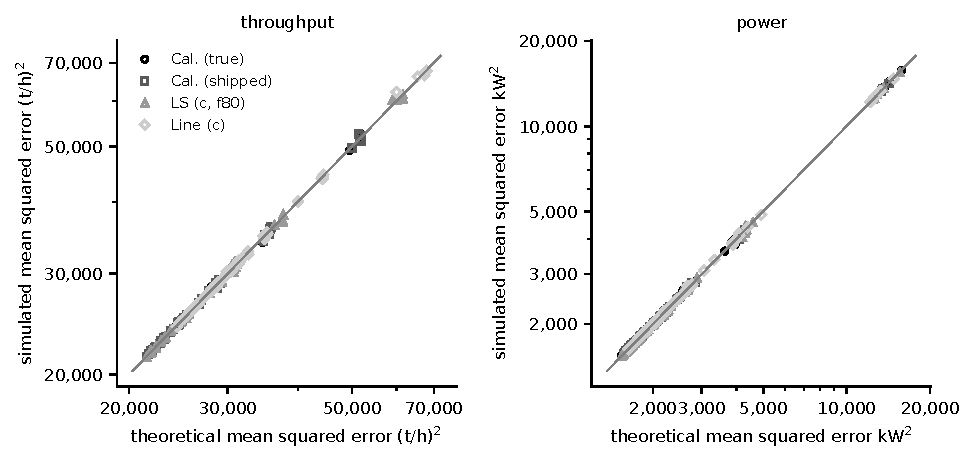
\includegraphics[width=\textwidth]{fig-theory-check}
\caption{Simulated against theoretical mean squared error for the four predictors with a closed-form risk, in every cell of the
study: throughput (left) and power (right). The theoretical value is Theorem~\ref{thm:risk} averaged over each replicate's test
points; the grey line is the identity. The largest of the \zNum{} absolute $z$ scores is \zMax.}
\label{fig:theory-check}
\end{figure*}

\subsection{Curvature alignment}\label{sec:results-align}

The plant V1 puts a share $\alpha$ of the engine's own power curvature into the plant, so Corollary~\ref{cor:align} predicts a
curvature gain $C=(2\alpha-1)\|e_0\|^2$ that changes sign at $\alpha=1/2$. Figure~\ref{fig:align} shows the paired difference of
squared error between the calibrated predictor with the true scalars and least squares, against $\alpha$. With 160 training
surveys the plane gain of Theorem~\ref{thm:fixed} has vanished and the difference is the curvature term alone: on the surveys
window it is $\alAmS$~kW$^2$ at $\alpha=-1$, $\alAhalfS$ at $\alpha=1/2$ and $\alAtwoS$ at $\alpha=2$, against theoretical values
of $-C$ of $-(\alCAmS)$, $-(\alCAhalfS)$ and $-(\alCAtwoS)$. The sign changes exactly at one half, on every design: the engine helps
when the plant carries more than half of the engine's curvature and hurts below. Under extrapolation the same alignment acts
with a larger amplitude ($\alAtwoX$~kW$^2$ at $\alpha=2$), because the test points lie where both curvatures are larger than in
the training window over which the fixed-design term is computed. Adding a curvature that the engine cannot follow,
V1(1, 2), leaves the gain where it was ($\alKqS$~kW$^2$ against $\alAoneS$ without it), as the corollary says: the orthogonal
part of the plant's curvature enters $\mathbf r$ but not $\langle e,r\rangle$.

With ten surveys the picture is different. The plane gain is $\alPlaneTen$~kW$^2$ on the surveys window, three times the
largest curvature gain, and the calibrated predictor beats least squares at every $\alpha$, even at $\alpha=-1$
($\alAmTen$~kW$^2$): with few surveys, what the engine contributes is a shrinkage target for the plane, and its curvature is a
second-order term. The size of the curvature itself bounds what it can ever contribute. The engine's power departs from a
plane in the setting and the feed size by \eRmsS~kW root mean square on the surveys window and \eRmsW~kW on the wide one,
against a noise of \sigKw~kW, so the curvature gain of a perfectly aligned engine ($\alpha=1$) is \curvShareKw\pct{} of the
noise variance. H1 held: the method beats least squares at small shrinkage if and only if the curvature term is positive.

\begin{figure}[!t]
\centering
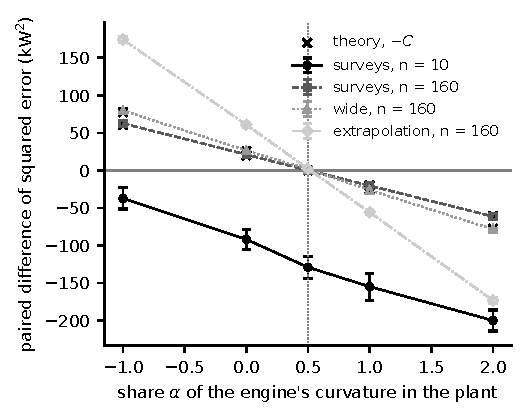
\includegraphics[width=\columnwidth]{fig-align}
\caption{Paired difference of squared error, calibrated predictor with the true scalars minus least squares, on the power of
the plants V1($\alpha$, 0), against the share $\alpha$ of the engine's curvature in the plant (negative: the calibration is
better). Bars: 95\pct{} Monte Carlo intervals over 1,900 replicates. Crosses: $-C$ of Theorem~\ref{thm:fixed} on the training
window. The dotted line marks $\alpha=1/2$.}
\label{fig:align}
\end{figure}

\subsection{Capacity: the affine and the curved forms}\label{sec:results-capacity}

On throughput the shipped engine is affine in the regressors, so by Corollary~\ref{cor:affine} its only contribution is the
shrinkage target. Figure~\ref{fig:capacity} shows the RMSE of the calibrated predictor relative to least squares for the three
engines of the capacity study, on the plant whose capacity is the power law of Rocha et al.~\cite{rocha}. With the affine engine
the ratio is \capAffSTen{} at ten surveys and \capAffSBig{} at 160 on the surveys window, the plane gain decaying as
Theorem~\ref{thm:fixed} predicts; under extrapolation from ten surveys it is \capAffXTen, the largest shrinkage benefit of the
study, and it too vanishes with the surveys (\capAffXBig). With the engine of the plant's own form the ratio stays below one
at 160 surveys: \capRoSBig{} on the surveys window, \capRoWBig{} on the wide one and \capRoXBig{} under extrapolation, a gain that
persists and grows with the width of the window and with the distance of the test points, as H2 stated. Its size is set by the
plant: the plant's capacity departs from a plane by \rRmsTph~t/h root mean square on the surveys window (\rRmsTphW{} on the wide
one) against a noise of \sigTph~t/h, so even an engine of exactly the right form can remove at most \curvCeilTph\pct{} of the
mean squared error.

The engine with half the exponents tests Corollary~\ref{cor:align} where the alignment is not built in. On the surveys window
its curvature is aligned ($\rho=\halfRhoS$) and smaller than the plant's ($\kappa=\halfKappaS$), so it gains
(\capHalfSBig); on the wide window its departure from the plane has another shape ($\rho=\halfRhoW$, $\kappa=\halfKappaW$, so
$\kappa>2\rho$) and it loses (\capHalfWBig), and more under extrapolation (\capHalfXBig). A curvature of the right sign is not
enough: what counts is its projection on the plant's departure from a plane, over the range where predictions are made. The
engine alone, refit without a discrepancy, is the best predictor when its form is exactly the plant's (\capRoRefitXTen{} of
the least-squares RMSE under extrapolation from ten surveys, \capRoRefitSBig{} at 160 on the surveys window) and the worst
when it is not (\capAffRefitSBig{} for the affine engine at 160): the discrepancy is insurance against a wrong form, and it
costs variance when the form is right.

The plant V2 runs the product's engine, with all eight scalars, against the same curved capacity and a power that follows it.
On throughput its result is the affine case: \rVtwoSTenTphOr~t/h for the calibration with the true scalars against
\rVtwoSTenTphLs{} for least squares and \rVtwoSTenTphLine{} for the line at ten surveys, a shrinkage gain only. On power the
engine's curvature is aligned with the plant's but too large ($\rho=\vtwoRho$, $\kappa=\vtwoKappa>2\rho$), the curvature term is
negative ($C=\vtwoC$~kW$^2$), and at 160 surveys the calibration is level with least squares (\rVtwoSBigKwOr{} against
\rVtwoSBigKwLs~kW) while at ten it still gains through the shrinkage (\rVtwoSTenKwOr{} against \rVtwoSTenKwLs). The engine
alone at the scalars of the $L_2$ projection predicts power best at ten surveys (\rVtwoSTenKwEngOr~kW). That projection is a
reference, not a converged optimum: the damped Gauss-Newton iteration reduced the weighted squared distance from \ltwoStart{}
to \ltwoEnd{} in \ltwoIters{} iterations, stopped at its iteration cap with three scalars on the bounds of their priors, and the
oracle predictors of V2 use the scalars where it stopped.

\begin{figure*}[!t]
\centering
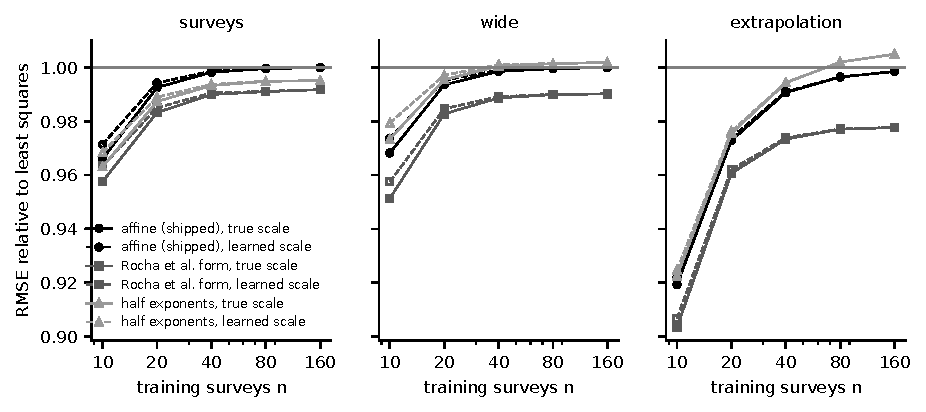
\includegraphics[width=\textwidth]{fig-capacity}
\caption{RMSE of the calibrated throughput predictor relative to least squares on the plant with the capacity law of Rocha et
al., against the number of training surveys, for three engines: the shipped affine capacity, the plant's own power-law form and
the same form with halved exponents; filled markers with the true scale, open markers with the scale learned in the linearized
model. Left to right: surveys window, wide window, extrapolation.}
\label{fig:capacity}
\end{figure*}

\subsection{Sample size, the setting-only line and the discrepancy scale}\label{sec:results-n}

Figure~\ref{fig:nsweep} shows the RMSE on V0 against the number of surveys. On throughput the feed size carries a large
signal beyond the setting ($\phi^2=\phiTwoTphS$~(t/h)$^2$ on the surveys window), so the crossing size of
Proposition~\ref{prop:line} is $n^\star=\nStarTphS$ and every regression on both regressors beats the line from ten surveys on
($\rVzeroSTenTphOr$ against $\rVzeroSTenTphLine$~t/h at $n=10$). On power the feed signal is small ($\phi^2=\phiTwoKwS$~kW$^2$),
the curvature gain is $C=\cFixKwS$~kW$^2$ and $n^\star=\nStarKwS$. The paired difference against the line is
$\lineOrTen$~kW$^2$ at ten surveys, a tie, then $\lineOrTwenty$ at twenty and $\lineOrForty$ at forty, for the predictor with
the true scalars. With the scalars learned the crossing moves later: $\lineKoTen$ at ten, $\lineKoTwenty$ at twenty, a tie, and
$\lineKoForty$ at forty. On the wide window the plane term of~\eqref{eq:line} is positive at ten surveys
($\planeTenKwW$~kW$^2$: the shrinkage pulls toward an engine plane far from the plant's) and the line wins
($\rVzeroWTenKwLine$ against $\rVzeroWTenKwOr$~kW), although $n^\star=\nStarKwW$; the proposition accounts for this through its
plane term, which the crossing size alone omits. H3 held with that qualification: the crossing size locates the overtaking
when the plane term is small, and the full expression~\eqref{eq:line} locates it in every cell. On the real design of the ten
surveys the line is the best predictor of the plant fitted to them ($\rVzeroRealKwLine$~kW against $\rVzeroRealKwOr$ for the
calibration with the true scalars and $\rVzeroRealKwKo$ with learned ones), which is what the held-out comparison
of~\cite{cb002} found on the real surveys.

\begin{figure*}[!t]
\centering
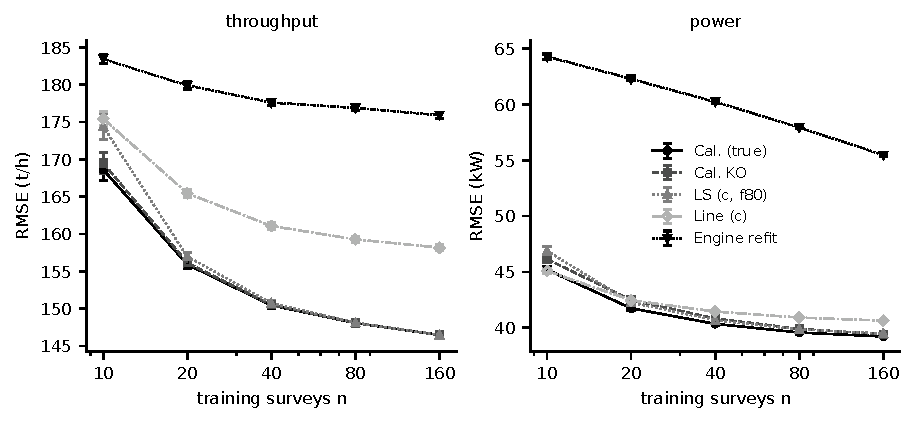
\includegraphics[width=\textwidth]{fig-nsweep}
\caption{RMSE against the number of training surveys on the plant V0 (the engine at the scalars fitted to the ten surveys plus
their fitted discrepancy) over the surveys window, for the calibrated predictor with the true and with the learned scalars,
least squares on the setting and the feed size, the line in the setting and the engine refit without a discrepancy; bars are
95\pct{} Monte Carlo intervals. Left: throughput; right: power.}
\label{fig:nsweep}
\end{figure*}

The discrepancy scale enters through $\lambda=\sigma^2/\tau^2$. Figure~\ref{fig:tau} gives the RMSE of the power prediction with
the true scalars against $\tau$, computed from Theorem~\ref{thm:risk} over 400 designs per size. The risk-optimal scale is
\tauBestTen~kW at ten surveys and \tauBestOneSixty~kW at 160, against the product's 36~kW, and the per-direction optima
of~\eqref{eq:taustar}, the mismatches $|\tilde\delta_k|$ of the engine's and the plant's planes, are \deltaOne, \deltaTwo{} and
\deltaThree~kW. The product's scale sits close to the largest of them and the curve is flat around its minimum:
\tauRmseProdTen~kW at 36 against \tauRmseBestTen~kW at the optimum, for ten surveys. The scale of the discrepancy prior is
therefore not what keeps the method from beating the line on ten surveys ($\tauRmseLineTen$~kW); the noise is.

\begin{figure}[!t]
\centering
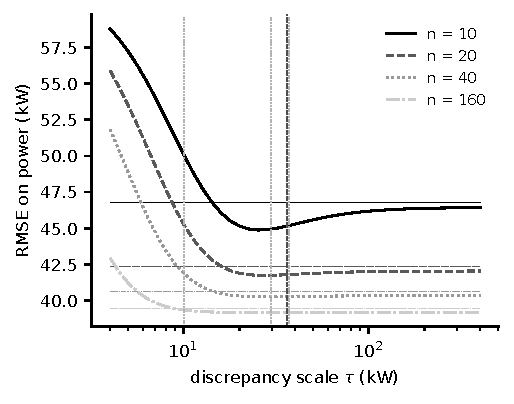
\includegraphics[width=\columnwidth]{fig-tau}
\caption{RMSE on the power of V0 of the calibrated predictor with the true scalars against the discrepancy scale $\tau$, for
four numbers of surveys (thick lines), with least squares at the same sizes (thin lines); dashed: the product's $\tau=36$~kW;
dotted: the plane mismatches $|\tilde\delta_k|$ of~\eqref{eq:taustar}. From Theorem~\ref{thm:risk} over 400 designs per size.}
\label{fig:tau}
\end{figure}

\subsection{The bands}\label{sec:results-bands}

Excluding one plant discussed below, the 80\pct{} band of the calibrated predictor with the true scalars covers between
\covOrMin{} and \covOrMax{} of the test points, with the learned scalars between \covKoMin{} and \covKoMax, and the Student-$t$
band of least squares between \covLsMin{} and \covLsMax. The exact coverage of Corollary~\ref{cor:coverage}, computed on the
plants V0 and V1 over 400 designs, lies between \covExactMin{} and \covExactMax, beside simulated values such as
\covOrSimRealKw{} on the real design and \covOrSimWTenKw{} on the wide window at ten surveys. The coverage falls below nominal
where the theorem places a bias, on the wide window and under extrapolation at small $n$, and the calibrated band stays narrower
than the least-squares band in every cell of Table~\ref{tab:main}. The engine refit without a discrepancy covers as little as
\covRefitMin{} of the test points (its band ignores its own model error), and the calibration at the shipped scalars covers
\covNomMin{} to \covNomMax. The exception is V1(1, 2) under extrapolation: the added curvature grows quadratically outside the
training window, and every band fails there (\covKqXOr{} for the calibration with the true scalars and \covKqXLs{} for least
squares at 160 surveys, \covKqXTenOr{} at ten). No predictor in the study can be trusted outside its training window against a
curvature it does not model.

\subsection{What a design identifies}\label{sec:results-design}

The ceiling of Proposition~\ref{prop:bound} is reached on the ten surveys. The throughput's information about $\ln
Q_{\mathrm{ref}}$ is \ceilInfo{} against the ceiling of \ceilBound{} and a prior precision of \ceilPrior; with throughput alone the
ratio of posterior to prior standard deviation could not fall below \ceilTphOnly. The linearized model with both outputs gives
\ceilLinTen{} on the ten surveys and the sampler of~\cite{cb002} measured \ceilMeasTen, while the floor~\eqref{eq:floor} that no
number of surveys at the fixed speed can pass is \ceilFloor: the ten surveys already give \ceilShare\pct{} of the narrowing of the
capacity base that any campaign at this speed could give. The power sensitivities to $\ln Q_{\mathrm{ref}}$, $\ln W_i$ and
$\ln\zeta$ agree to a relative \productRel, the structural product the floor rests on. Figure~\ref{fig:ceiling} shows the
saturation: \ceilSweepMax{} at \ceilSweepN{} surveys at the fixed speed and \ceilSweepVaried{} with the speed varied over 324,
360 and 396~rpm. Varying the speed does not break the ceiling, because the engine's capacity is flat at its optimum speed (the
factor $s e^{1-s}$ is within 0.6\pct{} of one at ten percent either way), so the sensitivity it moves out of the span of the
discrepancy is a fraction of a percent of the throughput.

\begin{figure}[!t]
\centering
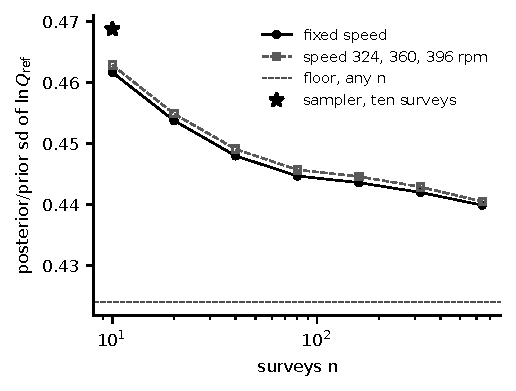
\includegraphics[width=\columnwidth]{fig-ceiling}
\caption{Ratio of posterior to prior standard deviation of the log capacity base against the number of surveys drawn from the
surveys window, in the linearized model with both outputs, at the fixed speed and with the speed varied (mean of 50 designs);
dashed: the floor~\eqref{eq:floor} for any number of surveys at the fixed speed; star: the sampler's value on the ten surveys.}
\label{fig:ceiling}
\end{figure}

Table~\ref{tab:design} and Figure~\ref{fig:design} rank the designs by the expected information gain~\eqref{eq:eig}. The ten
surveys give \eigDzero{} nats. Varying the speed gives \eigDtwo, twenty surveys \eigDthree{} and ten surveys over the wide window
\eigDfour. A measured product size with a noise of 2\pct{} of its mean ($\pEightyMean$~mm) gives \eigPtwo{} nats, more than
doubling the surveys, and at 5\pct{} noise it gives \eigPfive{}, as much as doubling them; at 10\pct{} \eigPten. The product
size is the output that reaches the population-balance scalars: the ratio of $s_{K_1}$ falls from \kOneDzero{} to \kOnePtwo, that
of $s_{K_2}$ to \kTwoPtwo, of $\Delta t_{10}$ to \tTenPtwo{} and of $K_3$ to \kThreePtwo, where throughput and power leave them
near their priors. Twenty surveys also narrow $s_{K_1}$ (\kOneDthree), through the wider spread of settings and feed sizes a
random design has against the ten surveys. H5 held for the product size and failed for the speed: within ten percent of the
capacity optimum, varying the speed teaches nothing that doubling the surveys does not teach better.

\begin{table*}[!t]
\caption{Expected information gain (nats) about the eight scalars and the ratio of posterior to prior standard deviation of
each, in the model linearized at the plant truth with both outputs and their discrepancies, for eight designs; random designs
are the mean of 200 draws. A ratio near one: the design leaves the scalar at its prior.}
\label{tab:design}
\centering\footnotesize
\begin{tabular}{@{}lrrrrrrrrr@{}}
\toprule
Design & EIG (nats) & $Q_{\mathrm{ref}}$ & $W_i$ & $\zeta$ & $P_n$ & $s_{K_1}$ & $s_{K_2}$ & $K_3$ & $\Delta t_{10}$ \\
\midrule
ten surveys (throughput, power) & 1.76 & 0.46 & 0.92 & 0.85 & 0.85 & 0.92 & 0.98 & 0.99 & 0.99 \\
ten surveys, speed 324 to 396 rpm & 1.76 & 0.46 & 0.92 & 0.85 & 0.85 & 0.92 & 0.98 & 0.99 & 0.99 \\
twenty surveys, surveys window & 2.14 & 0.45 & 0.92 & 0.85 & 0.85 & 0.67 & 0.97 & 0.99 & 0.99 \\
ten surveys, wide window & 1.92 & 0.46 & 0.92 & 0.85 & 0.85 & 0.78 & 0.98 & 0.99 & 1.00 \\
ten surveys and P80, noise 10\pct{} & 2.03 & 0.46 & 0.92 & 0.84 & 0.85 & 0.80 & 0.92 & 0.98 & 0.98 \\
ten surveys and P80, noise 5\pct{} & 2.16 & 0.46 & 0.92 & 0.84 & 0.85 & 0.72 & 0.91 & 0.98 & 0.97 \\
ten surveys and P80, noise 2\pct{} & 2.73 & 0.46 & 0.92 & 0.84 & 0.84 & 0.51 & 0.87 & 0.96 & 0.91 \\
P80 (2\pct{}) and varied speed & 2.72 & 0.46 & 0.92 & 0.84 & 0.84 & 0.51 & 0.87 & 0.96 & 0.91 \\
\bottomrule
\end{tabular}

\end{table*}

\begin{figure*}[!t]
\centering
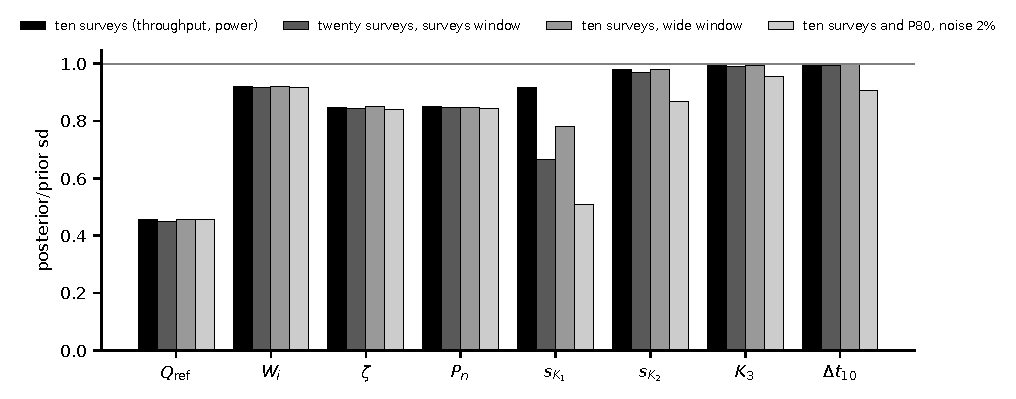
\includegraphics[width=\textwidth]{fig-design}
\caption{Ratio of posterior to prior standard deviation of each of the eight scalars for four designs: the ten surveys, twenty
surveys over the surveys window, ten surveys over the wide window, and the ten surveys with a product-size measurement of 2\pct{}
noise; linearized model at the plant truth. The product size is the only added output that reaches the classification and
breakage scalars.}
\label{fig:design}
\end{figure*}

\subsection{The full sampler}\label{sec:results-sampler}

\sbcText{}


\section{Ablation}\label{sec:ablation}

The calibrated predictor has four components that the study can switch one at a time: the scalars (given at the truth,
given at their shipped values, or learned), the discrepancy prior (Kennedy and O'Hagan, orthogonal or scaled), the
discrepancy itself (kept or dropped), and the form of the engine (affine or curved capacity). Table~\ref{tab:ablation} gives
the RMSE of each variant on six cells; the capacity form is the subject of Figure~\ref{fig:capacity} and is not repeated.

\begin{table}[!t]
\caption{Ablation of the calibrated predictor: RMSE (kW for power, t/h for throughput) on six cells with the scalars at the
truth, at their shipped values and learned under the three discrepancy priors, with the discrepancy dropped (the engine refit
alone), and least squares on the setting and the feed size for reference; \repsPerCell{} replicates per cell.}
\label{tab:ablation}
\centering\footnotesize
\resizebox{\columnwidth}{!}{\begin{tabular}{@{}lrrrrrrr@{}}
\toprule
Cell & True & Shipped & KO & Orth. & Scaled & No discr. & LS \\
\midrule
V0 power, surveys, 10 & 45.2 & 46.9 & 46.1 & 71.4 & 46.1 & 64.3 & 46.9 \\
V0 power, surveys, 160 & 39.2 & 39.5 & 39.4 & 49.3 & 39.4 & 55.4 & 39.5 \\
V0 tph, surveys, 10 & 168.6 & 168.6 & 169.5 & 169.4 & 167.4 & 183.5 & 174.4 \\
V2 tph, surveys, 10 & 168.1 & 168.2 & 169.0 & 168.9 & 167.1 & 186.2 & 173.7 \\
V2 power, extrap., 40 & 45.4 & 46.1 & 45.8 & 53.5 & 45.5 & 50.7 & 45.9 \\
V1($-1$) power, wide, 40 & 41.8 & 42.0 & 41.6 & 93.4 & 41.9 & 94.9 & 40.7 \\
\bottomrule
\end{tabular}
}
\end{table}

\subsection{The scalars}

Learning the scalars costs little against knowing them. On the power of V0 at ten surveys the predictor with the true scalars
reaches \rVzeroSTenKwOr~kW, the shipped scalars \rVzeroSTenKwNom{} and the learned ones \rVzeroSTenKwKo; at 160 surveys the
three are within half a kilowatt of one another and of least squares. On throughput the scalars hardly matter at all, because
the engine's throughput is affine and its scale is absorbed by the plane: the true and the shipped scalars give the same
\rVzeroSTenTphOr~t/h. The cost of learning the scalars is largest at ten surveys on the real design (\rVzeroRealKwKo{} against
\rVzeroRealKwOr~kW), where ten observations per output are shared between eight scalars, three discrepancy coefficients
and the noise; it is the price of the uncertainty that the band of the method carries and the residual band of a refit does not.
The learned predictor here is the linearized one, which fixes the noise scale at the plant's and drops the truncation of the
priors; Section~\ref{sec:results-sampler} measures the full posterior on the same replicates.

\subsection{The discrepancy prior}

The orthogonal prior is the costly change. With the product's proper priors on the scalars it raises the power RMSE on V0 from
\rVzeroSTenKwKo{} to \rVzeroSTenKwOrth~kW at ten surveys and from \rVzeroSBigKwKo{} to \rVzeroSBigKwOrth{} at 160, and on V1($-1$)
over the wide window to \rVamWFortyKwOrth~kW, next to the engine without a discrepancy (\rVamWFortyKwRefit). The mechanism is
Proposition~\ref{prop:priors}(a): the eight sensitivities of power on the training surveys span most of the directions of the
three discrepancy regressors, so the orthogonal complement leaves the discrepancy little room, and the plane the plant needs
must be carried by the scalars, whose priors forbid it. In the diffuse limit the two priors predict alike, by part (b); with the
priors the product uses, they do not, and the orthogonal prior behaves like the engine without a discrepancy. On throughput,
where only the capacity base has a sensitivity, the two priors are within a tenth of a percent of each other. The scaled prior
of Gu and Wang changes little on power on the surveys window (it is \scaledWideWorse\pct{} worse than the Kennedy and O'Hagan prior on
the wide window at ten surveys) and is the best of the three on throughput at ten surveys (\rVzeroSTenTphSc~t/h against
\rVzeroSTenTphKo{} for the Kennedy and O'Hagan prior), the shrinkage it adds along the well-measured directions being where the
throughput's plane mismatch is small. H4 as stated, that the priors change the risk less than they change the meaning of the
scalars, failed for the orthogonal prior: at proper priors it changes the risk most.

\subsection{The discrepancy}

Dropping the discrepancy is the largest change of all, in both directions. On every plant whose form the engine does not share
the refit engine is the worst predictor of the table except the orthogonal prior on two power rows, up to \rVamWFortyKwRefit~kW on V1($-1$) against \rVamWFortyKwLs{} for
least squares, and its band covers as little as \covRefitMin{} of the test points. On the capacity study with the engine of the
plant's own form it is the best predictor of the study (Section~\ref{sec:results-capacity}). The discrepancy plane therefore
buys robustness against a wrong form at the price of the variance of three coefficients, and Theorem~\ref{thm:fixed} prices
it: at most $3\sigma^2/n$ when the form is right, and the whole curvature of the plant when the form is wrong. The second price
is the larger on every plant of the study whose form the engine does not share, and the first fades with the surveys, so on
the evidence of this study the discrepancy should be kept unless the engine's form has been validated over the operating range
by other means; ten surveys of throughput and power cannot validate it.

\subsection{What the ablation says about the method}

Read together, the variants say that CrusherBayes is close to the best predictor available to it in every cell of the study
except one class: when the engine's form is exactly right, the discrepancy should be dropped, which no set of surveys can
establish in advance. Its band covers at about the nominal rate, as the Student-$t$ band of least squares does, and is the
narrower of the two in every cell of Table~\ref{tab:main}; its accuracy is that of least squares within the curvature and plane
terms of Theorem~\ref{thm:fixed}; and with learned scalars its RMSE is \rVzeroSTenKwKo~kW on ten random surveys against
\rVzeroSTenKwOr~kW with the true scalars, and \rVzeroRealKwKo{} against \rVzeroRealKwOr~kW on the real design. The choice of prior matters more than the choice of discrepancy scale, and the prior that the calibration literature
recommends for the meaning of the scalars is the wrong one for prediction with this engine.

\section{Discussion}\label{sec:discussion}

\subsection{Why the ten surveys could not separate the method from the line}

The held-out comparison of~\cite{cb002} found the method level with the line in the setting on power. The theory and the study
say why, term by term. The engine's throughput is affine, so on throughput the method is a ridge regression and its only gain
is the shrinkage of the plane, which is real at ten surveys but is a variance saving that a regression in both regressors
also mostly obtains. On power the engine's curvature over the range of the surveys is \eRmsS~kW against a noise of
\sigKw~kW, so even when it is perfectly aligned it removes \curvShareKw\pct{} of the noise variance. The feed size explains
little of the power beyond the setting ($\phi^2=\phiTwoKwS$~kW$^2$), so the third regressor of the discrepancy costs about as
much variance as it earns, and the crossing size $n^\star=\nStarKwS$ lies just above ten. On a virtual plant fitted to the ten
surveys, with the true scalars handed to it, the method ties the line at ten surveys ($\lineOrTen$~kW$^2$ in paired squared
error) and overtakes it from twenty on; with learned scalars from forty. A real campaign of ten surveys could not have shown a
difference that the theory says is a few kW$^2$ against a noise variance of about \sigKw$^2$.

\subsection{When the physics pays}

Corollary~\ref{cor:align} reduces the question to two numbers over the operating range of interest: the alignment $\rho$ of the
engine's departure from a plane with the plant's, and their relative size $\kappa$. Both can be estimated before a campaign.
The engine's departure $e$ is computable at any operating point. The plant's departure $r$ is not, but its size has a lower
bound in the scatter of past surveys about a plane, which contains the noise, and a sign that process knowledge often gives:
whether the capacity is concave or convex in the setting. The capacity of the engine used here is affine in the setting at the
fixed speed, so the physics in it cannot help predict throughput; a capacity law curved like the plant's, such as the power
law of Rocha et al.~\cite{rocha} or the concave capacity that Duarte et al.~\cite{duarte} measured on an HP400 over 6~mm of
setting, is the condition for any persistent gain on throughput. When the condition holds the gain persists as surveys
accumulate and grows under extrapolation, which is where the physics is meant to be used; its size is bounded by the plant's
own curvature relative to the noise, \curvCeilTph\pct{} of the squared error for the curvature the published capacity law gives
over the surveys window.

The second lesson is that the discrepancy prior is a predictive decision. Theorem~\ref{thm:fixed} gives the risk-optimal scale
in closed form, and on the plant fitted to the ten surveys the product's scale is close to it. The orthogonal prior, introduced
to give the scalars a meaning, takes the room of the discrepancy away when the engine has more sensitivities than the
discrepancy has regressors, and its predictions degrade toward those of the engine without a discrepancy. A practitioner who
wants interpretable scalars and good predictions can calibrate twice, with the orthogonal prior for the scalars and with the
standard prior for the predictions, as Proposition~\ref{prop:priors}(a) shows both are the same linear model with different
penalties.

\subsection{What to measure next}

The design study answers the question the earlier paper left open, which measurement would teach the scalars most. A product
size measured with a noise of 2 to 5\pct{} is worth as much as doubling the campaign or more, and it is the only added output
that reaches the classification and breakage scalars, which throughput and power leave near their priors. More surveys at the
same speed cannot narrow the capacity base below the floor of~\eqref{eq:floor}, which the ten surveys already approach
(\ceilShare\pct{} of the possible narrowing), and varying the speed by ten percent around the engine's capacity optimum adds
nothing, because the capacity is flat there. A design that moved the capacity base would need a factor that changes the
capacity outside the span of the discrepancy regressors by an amount comparable to the noise, which the speed does not do on
this engine; the study did not evaluate other factors. For prediction rather than identification, the cheapest improvement is
the noise itself: every gain of the method is measured against $\sigma^2$, so a better estimate of the throughput than the feed
rate of a survey, or of the power than the one estimated from the motor current, raises both the curvature and the plane gain in
proportion.

\subsection{Negative results}

Three hypotheses failed in part. The speed clause of H5 failed for the reason just given. H4 failed for the orthogonal prior,
which changes the risk more than any other component except the discrepancy itself. And the engine with half the exponents of
the plant's capacity law, a curvature of the right sign, lost to least squares on the wide window: the sign of a curvature does
not decide the gain, its projection on the plant's curvature over the prediction range does. Each of these is a statement about
this engine and these plants; each follows from a result of Section~\ref{sec:theory} that holds generally. The study also
confirms the negative result of~\cite{cb002} rather than overturning it: on a virtual plant built from the fit to the ten
surveys, with the scalars handed to it and the noise known, the method still ties the line at ten surveys. No change of prior,
scale or sampler would have changed the earlier comparison; only more surveys, less noise or an engine with a curved capacity
would.

\section{Limitations}\label{sec:limitations}

\subsection{Internal validity}

The theory holds conditionally on the scalars and on the design. The study measures the learning of the scalars in two ways,
the linearized model and the full sampler, and the second only on three cells with 50 replicates each, because one full
posterior costs about \cbCpuHours~CPU-hours at the product's size. The closed forms use the plant's noise scale, which the full
method learns; the verification cells measure what that costs. The linearization is taken at the prior centre, which is the
shipped engine, and the virtual plants put the truth at the posterior mean of the ten surveys, a distance of up to one prior
standard deviation on the power scalars; a plant further from the prior centre would make the linearized predictor worse and
the verification would have to be repeated there. The orthogonal prior is implemented in its empirical form over the training
surveys, which is the finite-dimensional form of the orthogonality of Plumlee~\cite{plumlee} with respect to the empirical
distribution of the operating points; a version orthogonal with respect to the operating window as a whole would differ by
the difference between the two distributions. The scaled prior is used with one value of its scaling constant. The Student-$t$
bands of the regressions use the residual variance and are exact under Gaussian noise; the Gaussian bands of the closed forms
use the true noise scale, which favours them.

\subsection{External validity}

The virtual plants are models. V0 and V1 are built from the engine itself, so their curvature is the engine's curvature,
scaled; V2 uses the capacity law that Rocha et al.~\cite{rocha} fitted to the same ten surveys, which is curved in the setting
with the exponent 1.27 their Table~4 prints, and which is itself a fit. The study therefore says when the method can win,
and by how much, on plants that curve as these do; it does not say that a given industrial crusher curves this way. A
three-point series of an HP400 in the work of Duarte et al.~\cite{duarte} shows a capacity concave in the setting over 6~mm,
which is evidence that real capacities can curve, not a measurement of how much. No discrete-element simulation is used as a
truth: one operating point of a quarter section of a secondary cone crusher took 172 to 404 CPU-hours~\cite{quistthesis}, and
the study needs thousands. The throw and the speed of the HP500 are held at 34~mm and 360~rpm, product assumptions for which no
primary source was found; the design with varied speed moves it by ten percent either way around the engine's capacity
optimum, and its conclusion depends on that range.

\subsection{Construct validity}

The risk is the mean squared error of a point prediction, and the comparison with the empirical predictors is made on it and
on the mean absolute percentage error; a decision that weighs an overprediction of power differently from an underprediction
would need another loss, under which Theorem~\ref{thm:risk} still gives the error's law under Gaussian noise but not the
ranking. The band is judged by its coverage and its width at the 80\pct{} level only. The discrepancy is a plane in two
regressors, as in the released method; a Gaussian-process discrepancy would change Proposition~\ref{prop:bound} (its kernel
would absorb curved sensitivities too) and the results of Section~\ref{sec:results-capacity}. The plants assume one ore and one
machine state across the surveys; a drift of the ore's hardness or of the liners' wear between surveys is a regressor that
neither the plant nor the predictors carry, and in a real set of surveys it would enter the noise and lower every gain measured here.

\section{Reproducibility}\label{sec:repro}

Every number, table and figure of this paper is computed from the files of the repository~\cite{chancadem} at release
\productrelease{} by committed scripts. The harness is \path{manuscripts/crusherbayes-theory/sim/}: \path{run_exact.py} runs
the closed-form study, \path{run_design.py} the design study and \path{run_sampler.py} the simulation-based calibration and the
verification; the identifiability analysis and the pilot are in \path{manuscripts/crusherbayes-theory/analysis/}; the
figures, the tables and the numbers of the text are written by \path{manuscripts/crusherbayes-theory/figures/make_figs.py}
from the summaries in \path{manuscripts/crusherbayes-theory/data/}. The tests of the harness, run with \texttt{pytest},
check the closed forms against the released implementation of the method, every identity of Section~\ref{sec:theory} on random
instances, and the independence of the results from the number of processes. The engine and the method are those of the
release, imported from \path{data-pipeline/pipeline/}; nothing in them was changed for this paper. The ten surveys are the
open table of Rocha et al.~\cite{rocha} (CC~BY~4.0), committed as \path{data/examples/hp500-surveys.csv}. The run times on the
machine of the study (\envCpus{} logical processors, \envPlatform, Python~\envPython, numpy~\envNumpy, emcee~\envEmcee), recorded
by \path{analysis/record_runs.py} in \path{data/run_times.json}, were \runExactTime{} for the closed-form study,
\runDesignTime{} for the design study, \runIdentTime{} for the identifiability analysis, \runTauTime{} for the analysis of the
discrepancy scale and the coverage, and \runSamplerTime{} for the full-sampler runs.

\section{Conclusions}\label{sec:conclusions}

Given its scalars, the prediction of a Bayesian calibration with a discrepancy linear in the regressors is least squares on
those regressors, shrunk toward the engine's plane, plus the engine's departure from that plane, and its risk has the exact form
of Theorem~\ref{thm:risk}. Over an empirical regression in the same regressors the engine gains in two ways: a shrinkage gain,
bounded by the variance of the fitted plane and fading with the number of surveys, and a curvature gain, which persists and is
positive only when the engine's curvature is aligned with the plant's and less than twice as large. On \cellsTotal{} cells of
virtual plants the theory matched the simulation to Monte Carlo error. For the HP500 engine of ChancaDEM the capacity is affine in
the setting, so on throughput only the shrinkage acts; on power the engine's curvature is \curvShareKw\pct{} of the noise
variance at best. A curved capacity of the plant's form gains a persistent \capRoRmseS{} to \capRoRmseW\pct{} of RMSE inside the
operating windows (\capRoMseS{} to \capRoMseW\pct{} of the mean squared error) and \capRoRmseX\pct{} under extrapolation, bounded
inside the training window by the plant's own curvature. The capacity base cannot be narrowed below a floor by more surveys at
the same speed over the same setting range, and a product-size measurement is the design that teaches the scalars most. The next steps are a product-size
measurement on the HP500 surveys, a capacity law curved in the setting inside the engine, and a discrepancy whose prior scale is
set by~\eqref{eq:taustar} rather than by convention.


\balance
% The reference list. Entries reused from the CrusherBayes 0.02 manuscript are copied verbatim; the new entries were
% resolved at Crossref or arXiv on 2026-11-19.
\begin{thebibliography}{00}

\bibitem{cochilco} Comisi\'on Chilena del Cobre (Cochilco), \emph{Consumo de energ\'ia en la miner\'ia del cobre,
actualizaci\'on a\~no 2024}. Santiago: Cochilco, 2025. [Online]. Available:
\url{https://www.cochilco.cl/web/download/991/2025/15151/consumo-de-energia-en-la-mineria-del-cobre-actualizacion-ano-2024.pdf}

\bibitem{whiten} W.~J. Whiten, ``The simulation of crushing plants with models developed using multiple spline
regression,'' \emph{Journal of the South African Institute of Mining and Metallurgy}, vol.~72, pp.~257--264, 1972; the
same paper in the APCOM 1972 proceedings, pp.~317--324. [Online]. Available: \url{https://www.saimm.co.za/Conferences/Apcom72/317-Whiten.pdf}

\bibitem{napier} T.~J. Napier-Munn, S.~Morrell, R.~D. Morrison, and T.~Kojovic, \emph{Mineral Comminution
Circuits: Their Operation and Optimisation}. Brisbane: Julius Kruttschnitt Mineral Research Centre, 1996. [Online].
Available: \url{https://search.worldcat.org/title/37081193}

\bibitem{bond} F.~C. Bond, ``The third theory of comminution,'' \emph{Transactions of the American Institute of
Mining, Metallurgical and Petroleum Engineers}, vol.~193, pp.~484--494, 1952. [Online]. Available:
\url{https://onemine.org/documents/the-third-theory-of-comminution}

\bibitem{rocha} B.~K.~N. da Rocha, T.~M. Campos, J.~Silva, and L.~M. Tavares, ``Fit-for-purpose model of HP500 cone
crusher in size reduction of itabirite iron ore,'' \emph{Minerals}, vol.~14, no.~9, art.~919, 2024.
doi:10.3390/min14090919.

\bibitem{duarte} R.~A. Duarte, A.~S. Yamashita, M.~T. da Silva, L.~P. Cota, and T.~A.~M. Euz\'ebio, ``Calibration and
validation of a cone crusher model with industrial data,'' \emph{Minerals}, vol.~11, no.~11, art.~1256, 2021.
doi:10.3390/min11111256.

\bibitem{yamashita} A.~S. Yamashita, A.~Thivierge, and T.~A.~M. Euz\'ebio, ``A review of modeling and control strategies
for cone crushers in the mineral processing and quarrying industries,'' \emph{Minerals Engineering}, vol.~170,
art.~107036, 2021. doi:10.1016/j.mineng.2021.107036.

\bibitem{quist} J.~Quist and C.~M. Evertsson, ``Cone crusher modelling and simulation using DEM,'' \emph{Minerals
Engineering}, vol.~85, pp.~92--105, 2016. doi:10.1016/j.mineng.2015.11.004.

\bibitem{ko} M.~C. Kennedy and A.~O'Hagan, ``Bayesian calibration of computer models,'' \emph{Journal of the Royal
Statistical Society: Series B}, vol.~63, no.~3, pp.~425--464, 2001. doi:10.1111/1467-9868.00294.

\bibitem{higdon} D.~Higdon, M.~Kennedy, J.~C. Cavendish, J.~A. Cafeo, and R.~D. Ryne, ``Combining field data and computer
simulations for calibration and prediction,'' \emph{SIAM Journal on Scientific Computing}, vol.~26, no.~2,
pp.~448--466, 2004. doi:10.1137/S1064827503426693.

\bibitem{bayarri} M.~J. Bayarri, J.~O. Berger, R.~Paulo, J.~Sacks, J.~A. Cafeo, J.~Cavendish, C.-H. Lin, and J.~Tu, ``A
framework for validation of computer models,'' \emph{Technometrics}, vol.~49, no.~2, pp.~138--154, 2007.
doi:10.1198/004017007000000092.

\bibitem{brynj} J.~Brynjarsd\'ottir and A.~O'Hagan, ``Learning about physical parameters: the importance of model
discrepancy,'' \emph{Inverse Problems}, vol.~30, no.~11, art.~114007, 2014. doi:10.1088/0266-5611/30/11/114007.

\bibitem{arendt} P.~D. Arendt, D.~W. Apley, and W.~Chen, ``Quantification of model uncertainty: calibration, model
discrepancy, and identifiability,'' \emph{Journal of Mechanical Design}, vol.~134, no.~10, art.~100908, 2012.
doi:10.1115/1.4007390.

\bibitem{tuowu} R.~Tuo and C.~F.~J. Wu, ``Efficient calibration for imperfect computer models,'' \emph{The Annals of
Statistics}, vol.~43, no.~6, pp.~2331--2352, 2015. doi:10.1214/15-AOS1314.

\bibitem{plumlee} M.~Plumlee, ``Bayesian calibration of inexact computer models,'' \emph{Journal of the American
Statistical Association}, vol.~112, no.~519, pp.~1274--1285, 2017. doi:10.1080/01621459.2016.1211016.

\bibitem{emcee} D.~Foreman-Mackey, D.~W. Hogg, D.~Lang, and J.~Goodman, ``emcee: The MCMC hammer,'' \emph{Publications of
the Astronomical Society of the Pacific}, vol.~125, no.~925, pp.~306--312, 2013. doi:10.1086/670067.

\bibitem{tb06} C.~J.~F. ter Braak, ``A Markov chain Monte Carlo version of the genetic algorithm differential evolution:
easy Bayesian computing for real parameter spaces,'' \emph{Statistics and Computing}, vol.~16, no.~3, pp.~239--249, 2006.
doi:10.1007/s11222-006-8769-1.

\bibitem{tbv08} C.~J.~F. ter Braak and J.~A. Vrugt, ``Differential evolution Markov chain with snooker updater and fewer
chains,'' \emph{Statistics and Computing}, vol.~18, no.~4, pp.~435--446, 2008. doi:10.1007/s11222-008-9104-9.

\bibitem{cb002} F.~Santib\'a\~nez-Leal, ``What ten industrial surveys identify in a cone-crusher population balance model:
Bayesian calibration with structural discrepancy narrows the engine's power band but gives no accuracy gain over a
setting-only line,'' preprint, version 0.02, Zenodo, 2026. doi:10.5281/zenodo.24243558.

\bibitem{chancadem} F.~Santib\'a\~nez-Leal, ``ChancaDEM: a crusher-comminution studio and a held-out evaluation of
cone-crusher models on ten industrial surveys,'' technical report, version 0.13.000, Zenodo, 2026.
doi:10.5281/zenodo.24243549.

\bibitem{quistthesis} J.~Quist, ``Cone crusher modelling and simulation,'' M.Sc. thesis, Department of Product and
Production Development, Chalmers University of Technology, Gothenburg, 2012. [Online]. Available:
\url{https://hdl.handle.net/20.500.12380/164816}

\bibitem{plumleejoseph} M.~Plumlee and V.~R. Joseph, ``Orthogonal Gaussian process models,'' \emph{Statistica Sinica},
2018 (online 2017). doi:10.5705/ss.202015.0404.

\bibitem{tuo} R.~Tuo, ``Adjustments to computer models via projected kernel calibration,'' \emph{SIAM/ASA Journal on
Uncertainty Quantification}, vol.~7, no.~2, pp.~553--578, 2019. doi:10.1137/17M1128769.

\bibitem{guwang} M.~Gu and L.~Wang, ``Scaled Gaussian stochastic process for computer model calibration and prediction,''
\emph{SIAM/ASA Journal on Uncertainty Quantification}, vol.~6, no.~4, pp.~1555--1583, 2018. doi:10.1137/17M1159890.

\bibitem{xiexu} F.~Xie and Y.~Xu, ``Bayesian projected calibration of computer models,'' \emph{Journal of the American
Statistical Association}, vol.~116, no.~536, pp.~1965--1982, 2021. doi:10.1080/01621459.2020.1753519.

\bibitem{wong} R.~K.~W. Wong, C.~B. Storlie, and T.~C.~M. Lee, ``A frequentist approach to computer model calibration,''
\emph{Journal of the Royal Statistical Society Series B}, vol.~79, no.~2, pp.~635--648, 2017. doi:10.1111/rssb.12182.

\bibitem{arendt2} P.~D. Arendt, D.~W. Apley, W.~Chen, D.~Lamb, and D.~Gorsich, ``Improving identifiability in model
calibration using multiple responses,'' \emph{Journal of Mechanical Design}, vol.~134, no.~10, art.~100909, 2012.
doi:10.1115/1.4007573.

\bibitem{sungtuo} C.-L. Sung and R.~Tuo, ``A review on computer model calibration,'' \emph{WIREs Computational Statistics},
vol.~16, no.~1, art.~e1645, 2024. doi:10.1002/wics.1645.

\bibitem{hsu} D.~Hsu, S.~M. Kakade, and T.~Zhang, ``Random design analysis of ridge regression,'' \emph{Foundations of
Computational Mathematics}, vol.~14, no.~3, pp.~569--600, 2014. doi:10.1007/s10208-014-9192-1.

\bibitem{hotvedt} M.~Hotvedt, B.~Grimstad, D.~Ljungquist, and L.~Imsland, ``When is gray-box modeling advantageous for
virtual flow metering?'' arXiv:2110.05034, 2021. [Online]. Available: \url{https://arxiv.org/abs/2110.05034}

\bibitem{woody} S.~Woody, N.~Ghaffari, and L.~Hund, ``Bayesian model calibration for extrapolative prediction via Gibbs
posteriors,'' arXiv:1909.05428, 2019. [Online]. Available: \url{https://arxiv.org/abs/1909.05428}

\bibitem{chaloner} K.~Chaloner and I.~Verdinelli, ``Bayesian experimental design: a review,'' \emph{Statistical Science},
vol.~10, no.~3, pp.~273--304, 1995. doi:10.1214/ss/1177009939.

\bibitem{ryan} E.~G. Ryan, C.~C. Drovandi, J.~M. McGree, and A.~N. Pettitt, ``A review of modern computational algorithms
for Bayesian optimal design,'' \emph{International Statistical Review}, vol.~84, no.~1, pp.~128--154, 2016.
doi:10.1111/insr.12107.

\bibitem{rainforth} T.~Rainforth, A.~Foster, D.~R. Ivanova, and F.~Bickford Smith, ``Modern Bayesian experimental design,''
\emph{Statistical Science}, vol.~39, no.~1, pp.~100--114, 2024. doi:10.1214/23-STS915.

\bibitem{huan} X.~Huan and Y.~M. Marzouk, ``Simulation-based optimal Bayesian experimental design for nonlinear systems,''
\emph{Journal of Computational Physics}, vol.~232, no.~1, pp.~288--317, 2013. doi:10.1016/j.jcp.2012.08.013.

\bibitem{raue} A.~Raue, C.~Kreutz, T.~Maiwald, J.~Bachmann, M.~Schilling, U.~Klingm\"uller, and J.~Timmer, ``Structural and
practical identifiability analysis of partially observed dynamical models by exploiting the profile likelihood,''
\emph{Bioinformatics}, vol.~25, no.~15, pp.~1923--1929, 2009. doi:10.1093/bioinformatics/btp358.

\bibitem{talts} S.~Talts, M.~Betancourt, D.~Simpson, A.~Vehtari, and A.~Gelman, ``Validating Bayesian inference algorithms
with simulation-based calibration,'' arXiv:1804.06788, 2018. [Online]. Available: \url{https://arxiv.org/abs/1804.06788}

\bibitem{modrak} M.~Modr\'ak, A.~H. Moon, S.~Kim, P.~B\"urkner, N.~Huurre, K.~Faltejskov\'a, A.~Gelman, and A.~Vehtari,
``Simulation-based calibration checking for Bayesian computation: the choice of test quantities shapes sensitivity,''
\emph{Bayesian Analysis}, vol.~20, no.~2, pp.~461--488, 2025. doi:10.1214/23-BA1404.

\bibitem{morris} T.~P. Morris, I.~R. White, and M.~J. Crowther, ``Using simulation studies to evaluate statistical
methods,'' \emph{Statistics in Medicine}, vol.~38, no.~11, pp.~2074--2102, 2019. doi:10.1002/sim.8086.

\bibitem{gelman} A.~Gelman, A.~Vehtari, D.~Simpson, C.~C. Margossian, B.~Carpenter, Y.~Yao, L.~Kennedy, J.~Gabry,
P.-C. B\"urkner, and M.~Modr\'ak, ``Bayesian workflow,'' arXiv:2011.01808, 2020. [Online]. Available:
\url{https://arxiv.org/abs/2011.01808}

\bibitem{hastie} T.~Hastie, R.~Tibshirani, and J.~Friedman, \emph{The Elements of Statistical Learning: Data Mining,
Inference, and Prediction}, 2nd~ed. New York: Springer, 2009. doi:10.1007/978-0-387-84858-7.

\bibitem{hoerl} A.~E. Hoerl and R.~W. Kennard, ``Ridge regression: biased estimation for nonorthogonal problems,''
\emph{Technometrics}, vol.~12, no.~1, pp.~55--67, 1970. doi:10.1080/00401706.1970.10488634.

\bibitem{mallows} C.~L. Mallows, ``Some comments on $C_p$,'' \emph{Technometrics}, vol.~15, no.~4, pp.~661--675, 1973.
doi:10.1080/00401706.1973.10489103.

\bibitem{diebold} F.~X. Diebold and R.~S. Mariano, ``Comparing predictive accuracy,'' \emph{Journal of Business \&
Economic Statistics}, vol.~13, no.~3, pp.~253--263, 1995. doi:10.1080/07350015.1995.10524599.

\end{thebibliography}


\end{document}
